\documentclass[floatfix,prb,aps,superscriptaddress,11pt]{revtex4}
\usepackage{amsfonts}
\usepackage{amsmath}
\usepackage{graphicx}
\usepackage{showlabels}
%\usepackage{showkeys}
\usepackage{color}
\usepackage{ulem}
\usepackage{subfigure}
\usepackage{bm}
%%%%% defs
%%%% acronimos
\def\copyr{$^\copyright$}
\def\reg{\textsuperscript{\textregistered}}
\def\tm{\textsuperscript{\texttrademark}}
\def\lufac{LUFAC${^\textsuperscript{\textregistered}}$}
%\def\depe{DP${^\textsuperscript{\texttrademark}}$}
\def\depe{DP${\texttrademark}$}
\def\ps{\mathrm{ps}}
\def\lda{\mathrm{LDA}}
\def\rpa{\mathrm{RPA}}
\def\nl{\mathrm{nl}}
\def\acu{Accu-Check\textsuperscript{\textregistered}~Performa}
\def\goni{Glucometro \'Optico No Invasivo}
\def\Reg{\textsuperscript{\textregistered}}
\def\tiniba{TINIBA\textsuperscript{\textregistered}}
\def\gw{{\it GW}}
\def\gsa{Generaci\'on del Segundo Arm\'onico}
\def\shg{Second Harmonic Generation}
\def\sfg{Sum Frequency Generation}
\def\sdf{Generaci\'on de Suma de Frecuencias}
%%%%% accent of i
\def\'#1{\if#1i{\accent19\i}\else{\accent19#1}\fi}
%%%%% compa\~nias
\def\micro{{\it Supermicro}}
%%%%% lugares
\def\lou{Laboratorio de \'Optica Ultrar\'apida}
\def\roma{Universidad de Roma II}
\def\tor{``Tor Vergata''}
\def\pssb{Physica Satatus Solidi B}
\def\dti{Direcci\'on de Tecnolog\'{\i}a e Innovaci\'on}
\def\di{Direcci\'on de Investigaci\'on}
\def\dfa{Direcci\'on de Formaci\'on Acd\'emica}
\def\dg{Direcci\'on General}
\def\da{Direcci\'on Administrativa}
\def\ifug{Insituto de F\'isica de la U. de Guanajuato}
\def\icf{Instituto de Ciencias F\'isicas}
\def\unam{Universidad Nacional Aut\'onoma de M\'exico}
\def\uguille{Universidad del Nordeste, Argentina}
\def\fotonica{Departamento de Fotonica}
\def\grupo{Propiedades \'Opticas de Nano-Sistemas, Interfases y Superficies}
\def\grupoa{PRONASIS}
%\def\grupo{Propiedades \'Opticas de Superficies e Interfases y Sistemas Nanosc\'opicos}
%\def\grupoa{POSISNA}
\def\di{Direcci\'on de Investigaci\'on}
\def\dfa{Direcci\'on de Formaci\'on Acad\'emica}
\def\cio{Centro de Investigaciones en \'Optica}
\def\ciod{Centro de Investigaciones en \'Optica, León, Guanajuato.}
\def\Conacyt{Consejo Nacional de Ciencia y Tecnolog\'ia}
\def\Concyteg{Consejo  de Ciencia y Tecnolog\'ia del Estado de Guanajuato}
\def\conacyt{CONACyT}
\def\concyteg{CONCyTEG}
\def\lagos{Centro Universitario de los Lagos}
\def\udeg{Universidad de Guadalajara}
\def\dinv{Direcci\'on de Investigaci\'on}
\def\dop{Department of Physics}
\def\uoft{University of Toronto}
\def\ua{University of Texas at Austin}
\def\icf{Instituto de Ciencias Físicas, UNAM, Cuernavaca}
%%%%% gente
%% grupo
\def\gabriel{Gabriel Ramos Ortíz}
\def\ramon{Ram\'on~ Carriles~ Jaimes}
\def\ramonm{Ram\acute{o}n~ Carriles~ Jaimes}
\def\enrique{Enrique~ Castro~ Camus}
\def\raul{Ra\'ul Alfonso V\'azquez Nava}
\def\raulm{Ra\acute{u}l~ Alfonso~ V\acute{a}zquez~ Nava}
\def\beto{Norberto~ Arzate~ Plata}
\def\bmsa{Bernardo S. Mendoza}
\def\bms{Bernardo~ Mendoza~ Santoyo}
%% alumnos
\def\cesar{C\'esar Castillo Quevedo}
\def\cabellos{Jos\'e Luis Cabellos Quiroz}
\def\tona{Tonatiuh Rangel Gordillo}
\def\temok{Juan Cuauhtemoc Salazar Gonz\'alez}
\def\adan{Luis Adan Mart\'inez Jim\'enez}
\def\sean{Sean Martin Anderson}
\def\reinaldo{Reinaldo Zapata Pe\~na}
\def\miguel{Miguel Angel Honorato Colin}
\def\oscar{Oscar Andrés Naranjo Montoya}
%%% alumnos del grupo
%% enrique
%Maestria:
\def\jorgee{Jorge Alberto Caballero Mendoza}
\def\sofia{Sofía Carolina Corzo García}
\def\ruth{Ruth Julieta Medina López} 
%Doctorado: 
\def\juane{Juan Jes\'us S\'anchez S\'anchez}
%Licenciatura
\def\alma{Alma Gabriela González Patlán}
%(con Ramon): 
\def\sergioer{Sergio Augusto Romero Serv\'{\i}n}
%% Raul
%Maestria:
\def\ramses{Ramses Valente Salazar Aparicio}
\def\enriquer{Enrique Arag\'on Navarro}%udg
\def\salomonr{Salom\'on Rodr\'{\i}guez Carrera}
\def\hectorr{H\'ector Santiago Hern\'andez}
\def\victor{Victor Manuel Villanueva Reyes}
%% Ramon
%Maestria:
\def\alfredora{Alfredo Campos Mej\'{\i}a}
%% Beto
%Doctorado
\def\noe{No\'e Gonz\'alez Baquedano}
%% otros
\def\mochan{W. Luis Mochán Backal}
\def\liliana{Liliana Wilson Herr\'an}
\def\gerardo{Gerardo E. S\'anchez Garc\'{\i}a Rojas}
\def\amalia{Amalia Mart\'inez Garc\'{\i}a}
\def\gabriel{Gabriel Ramos Ort\'{\i}z}
\def\nacho{Ing. José Ignacio Diego Manrique}
\def\tere{Teresita del Niño Jesús Pérez Hernández}
\def\elder{Elder de la Rosa Cruz}
\def\gonzalo{Gonzalo P\'aez Padilla}
\def\wlm{W. Luis Moch\'an Backal}
\def\oracio{Oracio C. Barbosa Garc\'ia}
\def\hector{H\'ector Hugo S\'anchez Hern\'andez}
\def\marco{Marco Antonio Escobar-Acevedo}
\def\gil{Alejandro Gil-Villegas Montiel}
\def\ernesto{Ernesto Carlos Cort\'es Morales}
\def\fms{Fernando Mendoza Santoyo}
\def\cuevas{Francisco Javier Cuevas de la Rosa}
\def\brenda{Brenda Esmeralda Matr\'inez Z\'erega}
\def\guille{Guillermo Ortiz}
\def\cesar{Cesar Castillo Quevedo}
\def\sipe{Prof. John Sipe}
\def\mike{Prof. Michael Downer}
\def\jems{Jorge Enrique Mej\'ia S\'anchez}
\def\lamon{Ram\'on Rodr\'iguez Vera}
\def\ldp{Luis de la Pe\~na}
\def\sole{Rodolfo Del Sole}
\def\lucia{Lucia Reining}
\def\sch{Schr\"odinger}
\def\Cuevas{Francisco J. Cuevas de la Rosa}
%%%%% categorias
\def\ita{Investigador Titular A}
\def\itb{Investigador Titular B}
\def\itc{Investigador Titular C}
\def\itd{Investigador Titular D}
\def\ite{Investigador Titular E}
\def\sr{Senior Researcher}
\def\iac{Investigador Asociado C}    
\def\alm{Alumno de Maestr\'ia}
\def\ald{Alumno de Doctorado}
\def\all{Alumno de Licenciatura}
\def\adei{Asistente de Investigaci\'on}
\def\sniIII{S.N.I. nivel III}
\def\sni{S.N.I.}
\def\cv{Currículum Vitae}
%%%%%% fonts
\def\tit{\sf}
\def\col{\sc}
\def\alu{\it} % for students
\def\cual{2$^{do}$}
\def\anno{2005}
\def\spe{\vspace{.12cm}}
%%%%%% cosas
\def\capa{capa-a-capa}
\def\espin{espintr\'onica}
\def\oespin{optoespintr\'onica}
\def\proyecto{Photon Assisted Spintronics}
\def\npro{48915}
\def\cvk{cv\mathbf{k}}
\def\cvkp{c'v'\mathbf{k}'}
%%%%%% revistas
\def\prb{Physical Review B}
\def\prl{Physical Review Letters}
\def\ol{Optics Letters}
\def\opn{Optics and Photonics News}
\def\pssc{physica status solidi (c)}
%%%%%%%%%%%%%%%%%%%%%%%%%%%%%%%%%%%%%%%
%%%%%% griegas
\def\ga{\alpha}
\def\gb{\beta}
\def\gga{\gamma}
\def\gGa{\Gamma}
\def\go{\omega}
\def\got{\tilde\omega}
\def\gO{\Omega}
\def\gr{{\rho}}
\def\ge{\epsilon}
\def\ve{\varepsilon}
\def\gve{\varepsilon}
\def\gd{\delta}
\def\gD{\Delta}
\def\gl{\lambda}
\def\gs{\sigma}
\def\gS{\Sigma}
\def\gbs{\overline{\sigma}}
\def\gka{\kappa}
%%%%%% griegas with tilde
\def\gta{\tilde{\alpha}}
\def\gtb{\tilde{\beta}}
\def\gtga{\tilde{\gamma}}
\def\gto{\tilde{\omega}}
\def\gtO{\tilde{\Omega}}
\def\gtr{\tilde{\rho}}
\def\gte{\tilde{\epsilon}}
\def\vte{\tilde{\varepsilon}}
\def\gtd{\tilde{\delta}}
\def\gtD{\tilde{\Delta}}
\def\gtl{\tilde{\lambda}}
\def\gts{\tilde{\sigma}}
\def\gtS{\tilde{\Sigma}}
%%%%%% romans with tilde
\def\bftr{\tilde{\mathbf{r}}}
\def\bftp{\tilde{\mathbf{p}}}
\def\bftv{\tilde{\mathbf{v}}}
\def\ta{\tilde{a}}
\def\tb{\tilde{b}}
\def\tr{\tilde{r}}
\def\tp{\tilde{p}}
\def\tV{\tilde{V}}
\def\tv{\tilde{v}}
%%
\newcommand{\ham}{\hat{\mathcal H}}
%%%%%% bra kets
\newcommand{\la}{\langle}
\newcommand{\ra}{\rangle}
\newcommand{\ket}[1]{| #1 \rangle}
\newcommand{\bra}[1]{\langle #1 |}
\newcommand{\braket}[2]{\langle {#1} | {#2} \rangle}
\newcommand{\ketbra}[2]{| {#1} \rangle {#1} \langle {#2} |}
\newcommand{\ave}[1]{\langle {#1} \rangle}
\newcommand{\dotp}[2]{\mathbf{#1} \cdot \mathbf{#2}}
%%%%%% averages
\newcommand{\prom}[1]{\langle {#1} \rangle}
%%%%%% creation and annihilation operators
\newcommand{\oa}{\hat a^{\tiny\strut}}
\newcommand{\oad}{\hat a^\dagger}
\newcommand{\oadk}{\hat a^\dagger_{\mathbf k}}
\newcommand{\oak}{\hat a^{\tiny\strut}_{\mathbf k}}
\newcommand{\obd}[1]{\hat b^\dagger_{#1}}
\newcommand{\ob}[1]{\hat b^{\tiny\strut}_{#1}}
%%%%%% Caligraphic
\newcommand{\cala}{{\cal A}}
\newcommand{\calb}{{\cal B}}
\newcommand{\calc}{{\cal C}}
\newcommand{\cald}{{\cal D}}
\newcommand{\cale}{{\cal E}}
\newcommand{\calf}{{\cal F}}
\newcommand{\calh}{{\cal H}}
\newcommand{\cali}{{\cal I}}
\newcommand{\calp}{{\cal P}}
\newcommand{\calg}{{\cal G}}
\newcommand{\calv}{{\cal V}}
\newcommand{\call}{{\cal L}}
\newcommand{\calo}{{\cal O}}
\newcommand{\calm}{{\cal M}}
\newcommand{\caln}{{\cal N}}
\newcommand{\calr}{{\cal R}}
\newcommand{\cals}{{\cal S}}
\newcommand{\calt}{{\cal T}}
\newcommand{\calu}{{\cal U}}
\newcommand{\calw}{{\cal W}}
\newcommand{\calbd}{\boldsymbol{\mathcal{\cal D}}}
\newcommand{\calbe}{\boldsymbol{\mathcal{\cal E}}}
\newcommand{\calbj}{\boldsymbol{\mathcal{\cal J}}}
\newcommand{\calbm}{\boldsymbol{\mathcal{\cal M}}}
\newcommand{\calbp}{\boldsymbol{\mathcal{\cal P}}}
\newcommand{\calbv}{\boldsymbol{\mathcal{\cal V}}}
\newcommand{\calbs}{\boldsymbol{\mathcal{\cal S}}}
\newcommand{\calbg}{\boldsymbol{\mathcal{\cal G}}}
%%%%%% mathematicla bold roman & greek
\newcommand{\mbf}[1]{\mathbf{#1}}
\newcommand{\mbg}[1]{\boldsymbol{\mathcal {#1}}}
\newcommand{\bfA}{\mathbf{A}}
\newcommand{\bfB}{\mathbf{B}}
\newcommand{\bfC}{\mathbf{C}}
\newcommand{\bfD}{\mathbf{D}}
\newcommand{\bfE}{\mathbf{E}}
\newcommand{\bfF}{\mathbf{F}}
\newcommand{\bfG}{\mathbf{G}}
\newcommand{\bfH}{\mathbf{H}}
\newcommand{\bfI}{\mathbf{I}}
\newcommand{\bfJ}{\mathbf{J}}
\newcommand{\bfK}{\mathbf{K}}
\newcommand{\bfL}{\mathbf{L}}
\newcommand{\bfM}{\mathbf{M}}
\newcommand{\bfN}{\mathbf{N}}
\newcommand{\bfP}{\mathbf{P}}
\newcommand{\bfR}{\mathbf{R}}
\newcommand{\bfS}{\mathbf{S}}
\newcommand{\bfT}{\mathbf{T}}
\newcommand{\bfU}{\mathbf{U}}
\newcommand{\bfV}{\mathbf{V}}
\newcommand{\bfW}{\mathbf{W}}
\newcommand{\bfX}{\mathbf{X}}
\newcommand{\bfY}{\mathbf{Y}}
\newcommand{\bfZ}{\mathbf{Z}}
\newcommand{\bfa}{\mathbf{a}}
\newcommand{\bfb}{\mathbf{b}}
\newcommand{\bfc}{\mathbf{c}}
\newcommand{\bfd}{\mathbf{d}}
\newcommand{\bfe}{\mathbf{e}}
\newcommand{\bff}{\mathbf{f}}
\newcommand{\bfg}{\mathbf{g}}
\newcommand{\bfh}{\mathbf{h}}
\newcommand{\bfi}{\mathbf{i}}
\newcommand{\bfj}{\mathbf{j}}
\newcommand{\bfk}{\mathbf{k}}
\newcommand{\bfn}{\mathbf{n}}
\newcommand{\bfp}{\mathbf{p}}
\newcommand{\bfq}{\mathbf{q}}
\newcommand{\bfr}{\mathbf{r}}
\newcommand{\bfs}{\mathbf{s}}
\newcommand{\bft}{\mathbf{t}}
\newcommand{\bfu}{\mathbf{u}}
\newcommand{\bfv}{\mathbf{v}}
\newcommand{\bfx}{\mathbf{x}}
\newcommand{\bfy}{\mathbf{y}}
\newcommand{\bfz}{\mathbf{z}}
\newcommand{\bfzero}{\mathbf{0}}
\newcommand{\bfone}{\mathbf{1}}
%
\newcommand{\bfgeta}{\boldsymbol{\eta}}
\newcommand{\bfSig}{\boldsymbol{\Sigma}}
\newcommand{\bfsig}{\boldsymbol{\sigma}}
\newcommand{\bfgS}{\boldsymbol{\Sigma}}
\newcommand{\bfgs}{\boldsymbol{\sigma}}
\newcommand{\bfga}{\boldsymbol{\alpha}}
\newcommand{\bfgb}{\boldsymbol{\beta}}
\newcommand{\bfge}{\boldsymbol{\epsilon}}
\newcommand{\bfgvare}{\boldsymbol{\varepsilon}}
\newcommand{\bfgg}{\boldsymbol{\gamma}}
\newcommand{\bfgG}{\boldsymbol{\Gamma}}
\newcommand{\bfgphi}{\boldsymbol{\phi}}
\newcommand{\bfgpsi}{\boldsymbol{\psi}}
\newcommand{\bfgD}{\boldsymbol{\Delta}}
\newcommand{\bfgPhi}{\boldsymbol{\Phi}}
\newcommand{\bfgPsi}{\boldsymbol{\Psi}}
\newcommand{\bfgtau}{\boldsymbol{\tau}}
\newcommand{\bfgxi}{\boldsymbol{\xi}}
\newcommand{\bfgchi}{\boldsymbol{\chi}}
\newcommand{\bfgnabla}{\boldsymbol{\nabla}}
\newcommand{\bfgnu}{\boldsymbol{\nu}}
\newcommand{\bfgmu}{\boldsymbol{\mu}}
\newcommand{\bfgrho}{\boldsymbol{\rho}}
\newcommand{\bfgRho}{\boldsymbol{\Rho}}
%%%%%% nabla
\newcommand{\nablak}{\frac{\partial}{\partial\mathbf{k}} }
%%%%%% ; derivative
\def\gk{{;\mathbf k}}
%%%%%% k derivative
\newcommand{\deriv}[2] {\frac{\partial {#1}} {\partial {#2} }}
%%%%%% prime for \sum
\def\prima{\strut^{_{'}}}
%%%%%% subindices
%\def\eti{n\bfk}
\newcommand{\eti}[1]{_{#1 \bfk}}
\newcommand{\etiup}[1]{_{#1 \bfk s}}
\newcommand{\etidn}[1]{_{#1 \bfk \bar{s}}}
%%%%% superindice to push down the subindex in greeks!
\def\pd{^{\strut}}
%%%%% gauges
\def\rde{$\bfr\cdot\bfE$~}
\def\rder{length-gauge}
\def\pda{$\bfp\cdot\bfA$~}
\def\vda{$\bfv\cdot\bfA$~}
\def\vdar{velocity-gauge}
%%%%% integral over k
\def\intk{\int\frac{d^3k}{8\pi^3}}
%%%%% roman indices
\def\rmi{\mathrm{i}}
\def\rmj{\mathrm{j}}
\def\rmk{\mathrm{k}}
\def\rml{\mathrm{l}}
\def\rmr{\mathrm{r}}
\def\rma{\mathrm{a}}
\def\rmb{\mathrm{b}}
\def\rmc{\mathrm{c}}
\def\rmd{\mathrm{d}}
\def\rme{\mathrm{e}}
\def\rmv{\mathrm{v}}
\def\rmz{\mathrm{z}}
\def\rmx{\mathrm{x}}
\def\rmy{\mathrm{y}}
\def\rmH{\mathrm{H}}
\def\rmI{\mathrm{I}}
\def\rmG{\mathrm{G}}
\def\rmW{\mathrm{W}}
%%%%% functions
\def\erf{\mathrm{erf}}
\def\erfc{\mathrm{erfc}}
\def\erfi{\mathrm{erfi}}

%iave: C01243171 y 0124317111
%%%%% Green's one point model
\def\tyv{\tilde y_v}
\def\ty{\tilde y}
\def\tv{\tilde v}

\def\ondip{/Users/bms/research/injection/paper/figures/all-fig}
%%%%%%%%%%%%%%%%%%%%%%%%%%%%%%%%%%%%%%%
\usepackage[backref,pdffitwindow,colorlinks,linkcolor={blue}]{hyperref}
%%%%%%%%%%%%%%%%%%%%%%%%%%%%%%%%%%%%%%%
\allowdisplaybreaks 
\begin{document}

\section{Notes on the derivation of $\mu^{abcd}$, $\zeta^{abc}$ and $\xi^{ab}$}

This notes start the day of August 16, 2016, for
$\mu^{\mathrm{abcd}}$, and contain the previous notes used for
$\zeta^{\mathrm{abc}}$ and $\xi^{\mathrm{ab}}$. 



\subsection{Multiple scale approach}
Using the multiple  scale  approach to solve the equation of motion for the single particle density matrix
$\rho_{nm}(\bfk;t)$, one can show that,\cite{nastosPRB07}
\begin{eqnarray}\label{rccp}
\frac{\partial\rho_{cc'}}{\partial  t}
&=&
-i \left(\omega_{cc'}-i\epsilon\right)
\rho_{cc'}
+\frac{e^2E^a(\omega)E^{b\star}(\omega)}{i\hbar^2}
\nonumber\\
&\times&
\sum_v
r^a_{cv}r^b_{vc'}
\left(
\frac{1}{\omega-\omega_{c'v}-i\epsilon}
-
\frac{1}
{\omega-\omega_{cv}+i\epsilon}
\right).
\end{eqnarray}
In order to proceed further, we take $\epsilon \rightarrow 0$  in the
first term, and then we change the density matrix operator to the so
called {\it interaction} representation, by which $\hat\rho$ is replaced
by 
\begin{equation}\label{rhoi}
\tilde{\hat{\rho}}=e^{iH_0t/\hbar}\hat\rho e^{-iH_0t/\hbar}
,
\end{equation}
with $H_0$ the ground state Hamiltonian.
The matrix elements are now,
\begin{eqnarray}\label{rhot}
\bra{c\bfk}
\tilde{\hat\rho}
\ket{c'\bfk}
&=&
\bra{c\bfk}
e^{iH_0t/\hbar}\hat\rho e^{-iH_0t/\hbar}
\ket{c'\bfk}
\nonumber\\
&=&
e^{i\omega_c t}
\bra{c\bfk}
\hat\rho
\ket{c'\bfk}
 e^{-i\omega_{c'}t}
\nonumber\\
\tilde\rho_{cc'}(\bfk) 
&=&
e^{i\omega_{cc'}t}
\rho_{cc'}(\bfk) 
,
\end{eqnarray}
where we used $H_0\ket{n\bfk}=\hbar\go_n(\bfk)\ket{n\bfk}$ with $\hbar\go_n(\bfk)$
the energy of the electronic band $n$ at point $\bfk$, and
$\ket{n\bfk}$ the Bloch state. The reciprocal lattice vector $\bfk$ is
restricted to the irreducible part of the first Brillouin zone. From
Eq.~\eqref{rhot} the
time derivative of $\tilde\rho_{cc'}(\bfk)$ is given by
\begin{eqnarray}\label{dtrho}
\frac{d\tilde\rho_{cc'}(\bfk)}{dt}
&=&
\Big(
i\omega_{cc'}
\rho_{cc'}(\bfk)
+
\frac{\partial\rho_{cc'}(\bfk)}{\partial t}
\Big)
e^{i\omega_{cc'}t}
\nonumber\\
&=&
\frac{e^2E^a(\omega)E^{b\star}(\omega)}{i\hbar^2}
e^{i\omega_{cc'}t}
\nonumber\\
&\times&
\sum_v
r^a_{cv}r^b_{vc'}
\left(
\frac{1}{\omega-\omega_{c'v}-i\epsilon}
-
\frac{1}
{\omega-\omega_{cv}+i\epsilon}
\right)
,
\end{eqnarray}
where we used Eq.~\eqref{rccp}, and the  $\epsilon \rightarrow 0$
still needs to be taken.

The expectation value of an observable ${\cal O}$ is given by
\begin{equation}\label{trace}
{\cal O}=\mbox{Tr}(\hat\rho\hat{\cal O})
,
\end{equation} 
where  Tr denotes the trace, given by the sum over the diagonal matrix
elements,
 and $\hat{\cal O}$ is the quantum
mechanical operator associated to the observable ${\cal O}$.
 Then,
\begin{eqnarray}\label{trace1}
{\cal O}
&=&
\int\frac{d^3k}{8\pi^3}
\sum_c
\bra{c\bfk}
\hat\rho\hat{\cal O})
\ket{c\bfk}
\nonumber \\
&=&
\int\frac{d^3k}{8\pi^3}
\sum_{cc'}
\bra{c\bfk}
\hat\rho
\ket{c'\bfk}
\bra{c'\bfk}
\hat{\cal O}
\ket{c\bfk}
\nonumber \\
&=&
\int\frac{d^3k}{8\pi^3}
\sum_{cc'}
\rho_{cc'}(\bfk)
{\cal O}_{c'c}(\bfk)
,
\end{eqnarray} 
where we used the closure relationship
$\sum_c\ket{c\bfk}\bra{c\bfk}=1$. In the interaction picture,
$\tilde{\cal O}_{c'c}=\bra{c'\bfk}
e^{iH_0t/\hbar}\hat{\cal O} e^{-iH_0t/\hbar}\ket{c\bfk}
={\cal O}_{c'c}e^{-i\omega_{cc'}t}$
and thus we can also write
\begin{eqnarray}\label{trace2}
{\cal O}
&=&
\int\frac{d^3k}{8\pi^3}
\sum_{cc'}
\tilde\rho_{cc'}(\bfk)
\tilde{\cal O}_{c'c}(\bfk)
,
\end{eqnarray} 
and so, we can calculate the expectation value using $\hat\rho$
 and $\hat{\cal O}$ in either the standard  Schr\"odinger
 representation or the
interaction representation. From the previous equation,
the rate of change of ${\cal O}$ is given by
From Eq.~\eqref{trace} we finally obtain that 
\begin{align}\label{0.e}
\frac{d\calo}{dt}
=\dot\calo=
\mathrm{Tr}(\frac{d\hat{{\tilde\rho}}}{dt}\tilde\calo) 
,
\end{align}
then,
\begin{eqnarray}\label{trace3}
\dot\calo  
&=&
\int\frac{d^3k}{8\pi^3}
\sum_{cc'}
\frac{d\tilde\rho_{cc'}(\bfk)}{dt}
\tilde{\cal O}_{c'c}(\bfk)  
\nonumber\\
&=&
\frac{e^2}{i\hbar^2}
\int\frac{d^3k}{8\pi^3}
\sum_{vcc'}
\calo_{c'c}r^a_{cv}r^b_{vc'}
\left(
\frac{1}{\omega-\omega_{c'v}-i\epsilon}
-
\frac{1}
{\omega-\omega_{cv}+i\epsilon}
\right)  
E^a(\omega)E^{b\star}(\omega)  
,
\end{eqnarray}   
where we used Eq.~\eqref{dtrho}, and we notice that the
$e^{i\go_{cc'}t}$
and $e^{-i\go_{cc'}t}$ factor cancel ecah other.


\subsection{Spin-current $\mu^{abcd}$}\label{sec:SC}

The operator for the spin current is given by
\begin{align}\label{1.e}
\hat\calo\to\hat K^{\rma\rmb}\equiv\hat v^\rma\hat S^\rmb  
,
\end{align} 
from where the matrix elements are
\begin{align}\label{2.e} 
K^{\rma\rmb}_{nm}
&=(\hat v^\rma\hat S^\rmb)_{nm} 
\nonumber\\ 
K^{\rma\rmb}_{nm}(\bfk)&=\sum_l v^\rma_{nl}(\bfk) S^\rmb _{lm} (\bfk)  
,
\end{align} 
by using $\sum_l\ket{l\bfk}\bra{l\bfk}=1$. Using time-reversal
invariance, from Sec.~\ref{sec:tr}, 
Eqs.~\eqref{en.41} and\eqref{en.43},
it
follows that,
$\bfv_{nm}(-\bfk)=-\bfv_{mn}(\bfk)$ and 
$\bfS_{nm}(-\bfk)=-\bfS_{mn}(\bfk)$, from where we obtain that 
\begin{align}\label{3.e} 
K^{\rma\rmb}_{nm}(-\bfk) 
&=\sum_l v^\rma_{nl}(-\bfk) S^\rmb _{lm} (-\bfk) 
=\sum_l (-v^\rma_{ln}(\bfk))(- S^\rmb _{ml} (\bfk) )  
\nonumber\\
&=\sum_l  
v^{\rma *}_{nl}(\bfk)  
S^{\rmb *} _{lm} (\bfk) 
=\sum_l 
(v^\rma_{nl}(\bfk)  
S^\rmb _{lm} (\bfk))^*=K^{\rma\rmb *}_{nm}(\bfk) 
.  
\end{align} 
From Eq.~\eqref{trace3}, using $\bfr_{nm}(-\bfk)=\bfr_{mn}(\bfk)$, and
taking $\epsilon\to 0$, we obtain,
\begin{align}\label{5.e}
\dot K^{\rma\rmb}
&=
\frac{e^2}{i\hbar^2}
\int\frac{d^3k}{8\pi^3}
\sum_{vcc'}
K^{\rma\rmb}_{c'c}
r^\rmc_{cv}r^\rmd_{vc'}
\left(
\frac{1}{\omega-\omega_{c'v}-i\epsilon}
-
\frac{1}
{\omega-\omega_{cv}+i\epsilon}
\right) 
E^\rmc(\omega)E^{\rmd\star}(\omega) 
\nonumber\\
&=
\frac{e^2}{i\hbar^2}
\int\frac{d^3k}{8\pi^3}
\sum_{vcc'}
\Big(
(K^{\rma\rmb}_{c'c}
r^\rmc_{cv}r^\rmd_{vc'}) \big |_{\bfk>0}
+
(K^{\rma\rmb}_{c'c}
r^\rmc_{cv}r^\rmd_{vc'}) \big |_{\bfk<0}
\Big) 
\nonumber\\
&\times 
\left(
\frac{1}{\omega-\omega_{c'v}-i\epsilon}
-
\frac{1}
{\omega-\omega_{cv}+i\epsilon}
\right) 
E^\rmc(\omega)E^{\rmd\star}(\omega) 
\nonumber\\
&=
\frac{e^2}{i\hbar^2}
\int_{\bfk>0}\frac{d^3k}{8\pi^3}
\sum_{vcc'}
\Big(
K^{\rma\rmb}_{c'c}
r^\rmc_{cv}r^\rmd_{vc'}
+
K^{\rma\rmb*}_{c'c}
r^\rmc_{vc}r^\rmd_{c'v}
\Big) 
\nonumber\\
&\times 
\left(
\frac{1}{\omega-\omega_{c'v}-i\epsilon}
-
\frac{1}
{\omega-\omega_{cv}+i\epsilon}
\right) 
E^\rmc(\omega)E^{\rmd\star}(\omega) 
\nonumber\\
&=
\frac{e^2}{i\hbar^2}
\int_{\bfk>0}\frac{d^3k}{8\pi^3}
\sum_{vcc'}
\Big(
K^{\rma\rmb}_{c'c}
r^\rmc_{cv}r^\rmd_{vc'}
+
(K^{\rma\rmb}_{c'c}
r^\rmc_{cv}r^\rmd_{vc'})^*
\Big) 
\nonumber\\
&\times 
\left(
\frac{1}{\omega-\omega_{c'v}-i\epsilon}
-
\frac{1}
{\omega-\omega_{cv}+i\epsilon}
\right) 
E^\rmc(\omega)E^{\rmd\star}(\omega) 
\nonumber\\
&=
\frac{e^2}{i\hbar^2}
\frac{1}{2}
\int\frac{d^3k}{8\pi^3}
\sum_{vcc'}
2\mathrm{Re}\Big[
K^{\rma\rmb}_{c'c}
r^\rmc_{cv}r^\rmd_{vc'}
\Big]
\Big\{
{\cal P}\left(
\frac{\go_{c'c}}{(\omega-\omega_{c'v})(\omega-\omega_{cv})}
\right) 
\nonumber\\
&+
i\pi 
\left(
\gd(\omega-\omega_{c'v}) 
+
\gd(\omega-\omega_{cv}) 
\right) 
\Big\}
E^\rmc(\omega)E^{\rmd\star}(\omega) 
\nonumber\\
&\approx 
\frac{\pi e^2}{\hbar^2}
\int\frac{d^3k}{8\pi^3}
\sum_{vcc'}
\mathrm{Re}\Big[
K^{\rma\rmb}_{c'c}
r^\rmc_{cv}r^\rmd_{vc'}
\Big]
\Big(
\gd(\omega-\omega_{c'v}) 
+
\gd(\omega-\omega_{cv}) 
\Big) 
E^\rmc(\omega)E^{\rmd\star}(\omega) 
\nonumber\\
&=
\frac{\pi e^2}{\hbar^2}
\int\frac{d^3k}{8\pi^3}
\sum_{vcc'}
\mathrm{Re}
\Big[ 
K^{\rma\rmb}_{c'c} 
r^\rmc_{cv}r^\rmd_{vc'}
+ 
K^{\rma\rmb}_{cc'} 
r^\rmc_{c'v}r^\rmd_{vc}
\Big]
\gd(\omega-\omega_{cv})  
E^\rmc(\omega)E^{\rmd\star}(\omega) 
,
\end{align} 
since $\go_{cc'}\sim 0$ and we exchange $c\leftrightarrow c'$. Now,
form Eq.~\eqref{3.e} we obtain that
\begin{align}\label{6.2}
\mathrm{Re}
\Big[ 
K^{\rma\rmb}_{cc'}
r^\rmc_{c'v}r^\rmd_{vc}
\Big]
&
=\frac{1}{2}\Big(
K^{\rma\rmb}_{cc'}
r^\rmc_{c'v}r^\rmd_{vc}
+
(K^{\rma\rmb}_{cc'}
r^\rmc_{c'v}r^\rmd_{vc})^*
\Big) 
\nonumber\\
&=\frac{1}{2}\Big(
K^{\rma\rmb}_{cc'}
r^\rmc_{c'v}r^\rmd_{vc}
+
K^{\rma\rmb}_{cc'}
r^\rmc_{vc'}r^\rmd_{cv}
\Big) 
=\mathrm{Re}
\Big[
K^{\rma\rmb}_{cc'}
r^\rmc_{vc'}r^\rmd_{cv}
\Big]
,
\end{align}
thus Eq.~\eqref{5.e} reduces to
\begin{align}\label{7.e}
\dot K^{\rma\rmb}
&=
\frac{\pi e^2}{\hbar^2}
\int\frac{d^3k}{8\pi^3}
\sum_{vcc'}
\mathrm{Re}
\Big[
K^{\rma\rmb}_{c'c}
r^\rmc_{cv}r^\rmd_{vc'}
+
K^{\rma\rmb}_{cc'}
r^\rmc_{vc'}r^\rmd_{cv}
\Big]
\gd(\omega-\omega_{cv}) 
E^\rmc(\omega)E^{\rmd\star}(\omega) 
\nonumber\\
&=
\frac{\pi e^2}{\hbar^2}
\int\frac{d^3k}{8\pi^3}
\sum_{vcc'}
\mathrm{Re}\Big[
K^{\rma\rmb}_{c'c}
\Big(
r^\rmc_{cv}r^\rmd_{vc'}
+
r^\rmd_{cv} r^\rmc_{vc'}
\Big) 
\Big]
\gd(\omega-\omega_{cv}) 
E^\rmc(\omega)E^{\rmd\star}(\omega) 
\nonumber\\
&=
\frac{\pi e^2}{\hbar^2}
\int\frac{d^3k}{8\pi^3}
\sum_{vcc'}
\mathrm{Re}\Big[
K^{\rma\rmb}_{c'c}
\Big(
r^\rmc_{cv}r^\rmd_{vc'}
+
(\rmc\leftrightarrow\rmd) 
\Big) 
\Big]
\gd(\omega-\omega_{cv}) 
E^\rmc(\omega)E^{\rmd\star}(\omega) 
\nonumber\\
&=
\frac{\pi e^2}{\hbar^2}
\int\frac{d^3k}{8\pi^3}
\sum_{vcc'}
\mathrm{Re}\Big[
K^{\rma\rmb}_{c'c}
\Big(
r^\rmc_{vc'} r^\rmd_{cv}
+
(\rmc\leftrightarrow\rmd) 
\Big) 
\Big]
\gd(\omega-\omega_{cv}) 
E^\rmc(\omega)E^{\rmd\star}(\omega) 
.
\end{align} 
We write
 \begin{align}\label{8.e}
\dot K^{\rma\rmb}
=
\mu^{\mathrm{abcd}} 
E^\rmc(\omega)E^{\rmd\star}(\omega) 
,
\end{align}
where from Eq.~\eqref{7.e} we obtain that
\begin{align}\label{9.e}
\mu^{\mathrm{abcd}}
&=
\frac{\pi e^2}{\hbar^2}
\int\frac{d^3k}{8\pi^3}
\sum'_{vcc'}
\mathrm{Re}\Big[ 
K^{\rma\rmb}_{c'c}
\Big( 
r^\rmc_{vc'} r^\rmd_{cv}
+
(\rmc\leftrightarrow\rmd) 
\Big) 
\Big]
\gd(\omega-\omega_{cv}) 
,  
\end{align}
where the $'$ in the sum, reminds us that $c$ and $c'$ are quasi
degenerate, and thus the sum only covers these states.
Above equation is the same as Eq. (3) of \cite{bhatPRL05}, which was
obtained by  using the semiconductor optical Bloch equations (SOBEs),
solved perturbatively to first order in the field intensity 
(H. Haug and S. W. Koch, Quantum Theory of the Optical
and Electronic Properties of Semiconductors (World Scientific,
Singapore, 1993); U. R\"ossler, Phys. Status Solidi B 234, 385 (2002)). 
  
From \onlinecite{andersonPRB15}, we include the scissors correction to
the band gap, and the nonlocal part of the pseudopotentials by taking
\begin{equation}
\mathbf{v}\equiv \dot{\mathbf{r}}=\frac{1}{i\hbar }[\mathbf{r},H_0],  
\label{mv}
\end{equation}
from where we define
\begin{align}
\mathbf{v}^\Sigma&=
\mathbf{v} 
+
\mathbf{v}^\mathrm{nl} 
+\mathbf{v}^S 
=
\mathbf{v}^\mathrm{LDA} 
+\mathbf{v}^S 
,
\label{vop2}
\end{align}
with
\begin{align}
\mathbf{v} 
&=\frac{\mathbf{p}}{m_e},
\nonumber\\
\mathbf{v}^\mathrm{nl} 
&=
\frac{1}{i\hbar}[\mathbf{r},V^\mathrm{nl}],\label{vnl}
\\
\mathbf{v}^S 
&=
\frac{1}{i\hbar}[\mathbf{r}, S],
\nonumber\\
\mathbf{v}^\mathrm{LDA} 
&=
\mathbf{v} 
+\mathbf{v}^\mathrm{nl}
.
\end{align}  
Then, 
\begin{align}\label{10.e}
\mu^{\mathrm{abcd}}
&=
\frac{\pi e^2}{\hbar^2}
\int\frac{d^3k}{8\pi^3}
\sum_{vcc'}
\mathrm{Re}\Big[ 
K^{\gS,\rma\rmb}_{c'c}
\Big( 
r^\rmc_{vc'} r^\rmd_{cv}
+
(\rmc\leftrightarrow\rmd) 
\Big) 
\Big]
\gd(\omega-\omega^\gS_{cv}) 
\nonumber\\
&=
\frac{\pi e^2}{2\hbar}
\int\frac{d^3k}{8\pi^3}
\sum_{vcc'}
\sum_l 
\mathrm{Re}\Big[ 
v^{\gS,\rma}_{c'l}\gs^\rmb_{lc}
\Big( 
r^\rmc_{vc'} r^\rmd_{cv}
+
(\rmc\leftrightarrow\rmd) 
\Big) 
\Big]
\gd(\omega-\omega^\gS_{cv}) 
,
\end{align} 
is the scissor corrected pseudotensor for the spin density injection
current that contains the contribution from the nonlocal part of the pseudopotentials,  
and is valid only for noncentrosymmetric crystals. 
We used,
\begin{align}\label{11.e}
K^{\gS,\rma\rmb}_{c'c}=\sum_lv^{\gS,\rma}_{c'l}S^\rmb_{lc}
=\frac{\hbar}{2}\sum_lv^{\gS,\rma}_{c'l}\gs^\rmb_{lc}
,
\end{align}
and $\go^\gS_{cv}=\go_c+\gD-\go_v$
includes the scissor corrected conduction energies, where $\gD$ is the
energy correction, and
\begin{equation}
\mathbf{r}_{nm}(\mathbf{k}) 
=
\frac{\mathbf{v}^\Sigma_{nm}(\mathbf{k})}{i\omega^\Sigma_{nm}(\mathbf{k})}
=
\frac{\mathbf{v}^\mathrm{LDA}_{nm}(\mathbf{k})}{i\omega^\mathrm{LDA}_{nm}(\mathbf{k})}
\quad\quad n\notin D_m 
, 
\label{chon.10}
\end{equation}
are the position matrix elements, which are the same in the scissored or
unscissored LDA case. We mention that $\bfr_{nm}(\bfk)$ contain the
contribution from the nonlocal part of the pseudopotential,
$V^{\mathrm{nl}}(\bfk)$.
\tiniba~codes $\bfv^{\gS}_{nm}(\bfk)$
under the array \verb=calVsig(3,nMax,nMax)=, where \verb=3= 
is
for the Cartesian directions ($1\to x,2\to y,3\to z$)  
and   \verb=nMax= is for the total number
of bands. This array works for bulk and surface calculations under the
same name; for a surface calculation it contains $\calbv^{\gS}_{nm}(\bfk)$.


\subsubsection{Units}

It so happens that in Gaussian (cgs) units (see Eq.~\eqref{trace53}) 
\begin{align}\label{rnn.n20}
[\mu]&=[v]
[\zeta]
\nonumber\\
[\mu_{\mathrm{S.I.}}]&=[v_{\mathrm{S.I.}}]
[\zeta_{\mathrm{S.I.}}]
\nonumber\\
\Rightarrow  
[\mu_{\mathrm{S.I.}}]&=\frac{m}{s}4\pi\frac{\hbar}{2}\frac{\ge_0}{\hbar}
[\mathrm{Im}[\chi_{\mathrm{cgs}}]]
,
\end{align}  
where we used Eq.~\eqref{rnn.n2}, and $\mathrm{Im}[\chi^{\rma\rmb}_{\mathrm{cgs}}]$ is  
dimensionless.  
Therefore, the units are 
\begin{align}\label{rnn.n3nn}
[\mu_{\mathrm{S.I.}}]&=\frac{m}{s}
[\hbar]\frac{[\ge_0]}{[\hbar]}
=\frac{m}{s} Js 
\frac{F/m}{Js}=\frac{m}{s} Js\frac{C/mV}{CVs}
=\frac{m}{s}
\frac{J}{mV^2}
=
\frac{J}{sV^2}
,
\end{align}
in agreement with Ref.~\onlinecite{nastosPRB07}, and with the units
derived  
from Eq.~\eqref{8.e}, i.e.
\begin{align}\label{zp.1}
[\dot K]&=[\mu][E]^2 
\nonumber\\
\frac{1}{s}\frac{m}{s}\hbar\frac{1}{m^3}
=
\frac{\hbar}{s^2m^2}
&=[\mu]
\frac{V^2}{m^2} 
\nonumber\\
\Rightarrow 
[\mu]&=\frac{\hbar}{s^2V^2}=\frac{J}{sV^2}
\nonumber\\
\Rightarrow 
[\dot K]&=\frac{J}{sm^2}
,
\end{align}  
where we recall that $\hat\bfS$ is the spin density.  
From Eqs.~\eqref{10.e} and \eqref{trace53},
and using Eq.~\eqref{rnn.n3}, we get
\begin{align}\label{um.1}
[\mu]&=
\frac{m}{s}
[\zeta]
=
\frac{m}{s}
\frac{J}{mV^2}
=
\frac{J}{sV^2}
,
\end{align} 
which agrees with Eq.~\eqref{rnn.n3nn}.


\subsection{Degree of Spin Injection}

From Sec.~\ref{sec:cir}, we can take Eq.~\eqref{rn}
\begin{equation}\label{rnn}
\dot n(\bfr)=\xi^{ab}(\bfr;\go) 
E^a(-\omega) E^b(\omega) 
,
\end{equation}
and define the degree of spin injection as 
\begin{align}\label{eez.1}
\calv^{\rma\rmb}\equiv\frac{\dot K^{\rma\rmb}}{(\hbar/2)\dot n}
,
\end{align}  
where as we se from Eqs.~\eqref{8.e}, \eqref{9.e}, \eqref{rn}  and
\eqref{xir}, the units are given by
\begin{align}\label{eez.1}
[\calv^{\rma\rmb}]
&=
\frac{[\dot K^{\rma\rmb}]}{(\hbar/2)[\dot n]}
\nonumber\\
&=
\frac{2}{\hbar}[v][S]=\frac{m}{s}
,
\end{align}
i.e. the degree of spin injection, $\calv^{\rma\rmb}$,
 gives the speed of an electron along the Cartesian direction
``$\rma$'', with a spin oriented along the Cartesian direction ``$\rmb$'',
in units of speed, i.e. $m/s$.


\subsubsection{Centrosymmetric Crystals}

For a centrosymmetric crystals, it follows that $H(\bfr)=H(-\bfr)$,
and that $\psi_n(\bfk,-\bfr)=\psi_n(-\bfk,\bfr)$
 (U.of.Toronto notes,
page 42), then 
\begin{align}\label{e.0}
\calo_{nm}(\bfk) 
&=\int d^3r\, \psi^*_n(\bfk,\bfr)\, \hat\calo(\bfr)\,\psi_m(\bfk,\bfr) 
\nonumber\\
\calo_{nm}(-\bfk) 
&=\int d^3r\, \psi^*_n(-\bfk,\bfr)\, \hat\calo(\bfr)\,\psi_m(-\bfk,\bfr) 
\nonumber\\
&=\int d^3r\, \psi^*_n(\bfk,-\bfr)\, \hat\calo(\bfr)\,\psi_m(\bfk,-\bfr) 
\nonumber\\
&=\int d^3r\, \psi^*_n(\bfk,\bfr)\,
  \hat\calo(-\bfr)\,\psi_m(\bfk,\bfr)\quad(\bfr\to-\bfr)  
\nonumber\\
&=\pm\int d^3r\, \psi^*_n(\bfk,\bfr)\,
  \hat\calo(\bfr)\,\psi_m(\bfk,\bfr)\quad(\calo(-\bfr)=\pm \calo(\bfr))  
\nonumber\\
&=\pm\calo_{nm}(\bfk)
.
\end{align}
Therefore, we obtain that
\begin{align}\label{e.1}
\bfr_{nm}(-\bfk)&=-\bfr_{nm}(\bfk) 
\nonumber\\
\bfv_{nm}(-\bfk)&=-\bfv_{nm}(\bfk) 
\nonumber\\
\bfS_{nm}(-\bfk)&=\bfS_{nm}(\bfk) 
,
\end{align}
since 
$\hat\bfr(-\bfr)=-\hat\bfr(\bfr)$,  
$\hat\bfv(-\bfr)=-\hat\bfv(\bfr)$  
and
$\hat\bfS(-\bfr)=\hat\bfS(\bfr)$, as the spin operator does not depend
on position. From Eq.~\eqref{3.e}
\begin{align}\label{e.2}
K^{\rma\rmb}_{nm}(-\bfk) 
&=\sum_l v^\rma_{nl}(-\bfk) S^\rmb _{lm} (-\bfk) 
=\sum_l (-v^\rma_{nl}(\bfk)) S^\rmb _{lm} (\bfk)
=-K^{\rma\rmb}_{nm}(\bfk) 
.
\end{align}
Now, 
\begin{align}\label{e.3}
(K^{\rma\rmb}_{c'c}
r^\rmc_{cv}r^\rmd_{vc'}) \big |_{\bfk<0}
=
-K^{\rma\rmb}_{c'c}
r^\rmc_{cv}r^\rmd_{vc'} \big |_{\bfk>0}
,
\end{align}
that when used in Eq.~\eqref{5.e}, would leads to
\begin{align}\label{e.4}
\mu^{\mathrm{abcd}}=0
%\quad\mathrm{for}\,\mathrm{Centrosymmetric}\,\mathrm{Crystals}  
,
\end{align}
for centrosymmetric crystals.
 

\subsection{Spin polarization $\zeta^{abc}$ and Degree of Spin Polarization}\label{sec:DSP} 
Eq. \eqref{trace3} can be used to compute the
\textit{spin-injection rate} 
$\dot{\bm{S}} \equiv\mathrm{d}\bm{S}/\mathrm{d}t$ with
\begin{eqnarray}\label{eq:Shat}
\hat{\cal O}\to
\hat{S}^a=\frac{\hbar}{2}\hat{\sigma}^a
\end{eqnarray}
where $\hat{\sigma}^a$ are the Pauli Matrices
\begin{eqnarray}\label{eq:pauliMatrix}
\hat\sigma^x=\left(\begin{array}{cc} 
0 & 1 \\ 
1 & 0  
\end{array}\right)  
,\quad  
\hat\sigma^y=\left(\begin{array}{cc} 
0  & -i \\ 
i & 0  
\end{array}\right)  
,\quad \text{and}\quad  
\hat\sigma^z=\left(\begin{array}{cc} 
1 & 0 \\ 
0 & -1  
\end{array}\right)  
\end{eqnarray} 
that are operators in spinor space, therefore, 
\begin{eqnarray}\label{trace4}
\frac{d{\cal S}^a}{dt}
&=&
\frac{e^2}{i\hbar^2}
\int\frac{d^3k}{8\pi^3}
\sum_{vcc'}
\hat{\cal S}^a_{c'c}r^b_{cv}r^c_{vc'}
\left(
\frac{1}{\omega-\omega_{c'v}-i\epsilon}
-
\frac{1}
{\omega-\omega_{cv}+i\epsilon}
\right)
E^b(\omega)E^{c\star}(\omega)
.
\end{eqnarray} 
Using the so called,%\cite{lax,najmaiePRB03} 
time-reversal invariance by which
\begin{eqnarray}\label{timer}
\go_m(-\bfk)&=&\go(\bfk),
\nonumber \\
r^a_{mn}(-\bfk)&=&r^a_{nm}(\bfk),
\nonumber \\
S^a_{mn}(-\bfk)&=&-S^a_{nm}(\bfk),
\end{eqnarray}
we can add the $\bfk$ and $-\bfk$ contributions to the integral in
Eq.~\eqref{trace4} to obtain 
\begin{eqnarray}\label{trace41}
\frac{d{\cal S}^a}{dt}
&=&
\frac{e^2}{i\hbar^2}
\int_{\bfk>0}\frac{d^3k}{8\pi^3}
\sum_{vcc'}
\Big(
\big(
{\cal S}^a_{c'c}r^b_{cv}r^c_{vc'}\big)|_{\bfk}
+
\big(
{\cal S}^a_{c'c}r^b_{cv}r^c_{vc'}\big)|_{-\bfk}
\Big)
\nonumber\\
&\times&
\left(
\frac{1}{\omega-\omega_{c'v}-i\epsilon}
-
\frac{1}
{\omega-\omega_{cv}+i\epsilon}
\right)
E^bE^{c\star}
\nonumber \\
&=&
\frac{e^2}{i\hbar^2}
\int_{\bfk>0}\frac{d^3k}{8\pi^3}
\sum_{vcc'}
\Big(
\big(
{\cal S}^a_{c'c}r^b_{cv}r^c_{vc'}\big)|_{\bfk}
-
\big(
\hat{\cal S}^a_{cc'}r^b_{vc}r^c_{c'v}\big)|_{\bfk}
\Big)
\nonumber\\
&\times&
\left(
\frac{1}{\omega-\omega_{c'v}-i\epsilon}
-
\frac{1}
{\omega-\omega_{cv}+i\epsilon}
\right)
E^bE^{c\star}
\nonumber \\
&=&
\frac{e^2}{i\hbar^2}
\frac{1}{2}\int\frac{d^3k}{8\pi^3}
\sum_{vcc'}
\Big(
{\cal S}^a_{c'c}r^b_{cv}r^c_{vc'}\big)
-
\big(
\hat{\cal S}^a_{c'c}r^b_{cv}r^c_{vc'}\big)^*
\Big)
\nonumber\\
&\times&
\left(
\frac{1}{\omega-\omega_{c'v}-i\epsilon}
-
\frac{1}
{\omega-\omega_{cv}+i\epsilon}
\right)
E^bE^{c\star}
\nonumber \\
&=&
\frac{e^2}{\hbar^2}
\int\frac{d^3k}{8\pi^3}
\sum_{vcc'}
\mbox{Im}\big[
{\cal S}^a_{c'c}r^b_{cv}r^c_{vc'}
\big]
%\nonumber\\
%&\times&
\left(
\frac{1}{\omega-\omega_{c'v}-i\epsilon}
-
\frac{1}
{\omega-\omega_{cv}+i\epsilon}
\right)
E^bE^{c\star}
,
\end{eqnarray} 
where in going from the second to the third equal sign, we use the
fact that for any Hermitian operator 
${\cal O}_{mn}(\bfk)={\cal O}^*_{nm}(\bfk)$, and that the one half
comes from the unrestricted integration over all values of $\bfk$ and
not only $\bfk>0$.
Aided by the identity
\begin{eqnarray}
  \label{eq:25}
\lim_{\epsilon\to 0}  \frac{1}{x\mp i\epsilon}=
\mathcal{P}(\frac{1}{x}) \pm
 i \pi\, \delta(x),
\end{eqnarray}
%\red{DUDA: [comment  something about principal parts]} 
where $\mathcal{P}$ means the \textit{principal part},
Eq.~\eqref{trace4} can be written as
\begin{eqnarray}\label{trace5}
\frac{d{\cal S}^a}{dt}
&=&
\frac{e^2}{\hbar^2}
\int\frac{d^3k}{8\pi^3}
\sum_{vcc'}
\mbox{Im}\big[
{\cal S}^a_{c'c}r^b_{cv}r^c_{vc'}
\big]
\Big\{
{\cal P}\left(
\frac{1}{\omega-\omega_{c'v}}
-
\frac{1}
{\omega-\omega_{cv}}
\right)
\nonumber\\
&+&
i\pi
\left(
\gd(\omega-\omega_{c'v})
+
\gd(\omega-\omega_{cv})
\right)
\Big\}
E^bE^{c\star}
\nonumber\\
&=&
\frac{e^2}{\hbar^2}
\int\frac{d^3k}{8\pi^3}
\sum_{vcc'}
\mbox{Im}\big[
{\cal S}^a_{c'c}r^b_{cv}r^c_{vc'}
\big]
\Big\{
{\cal P}\left(
\frac{\go_{c'c}}{(\omega-\omega_{c'v})(\omega-\omega_{cv})}
\right)  
\nonumber\\
&+& 
i\pi  
\left(
\gd(\omega-\omega_{c'v})  
+
\gd(\omega-\omega_{cv})  
\right)  
\Big\} 
E^bE^{c\star}
\nonumber\\
&\simeq&
\frac{i\pi e^2}{\hbar^2}
\int\frac{d^3k}{8\pi^3}
\sum_{vcc'}\phantom{}^\prime\,
\mbox{Im}\big[
{\cal S}^a_{c'c}r^b_{cv}r^c_{vc'}
\big]
\left(
\gd(\omega-\omega_{c'v})
+
\gd(\omega-\omega_{cv})
\right)
E^bE^{c\star}
,
\end{eqnarray}
since the term that goes with the principal part is of the order of
$\go_{cc'}$ which is very small as the states $c$ and $c'$ are quasi
degenerate. Indeed,
the primed sigma symbol $\Sigma^\prime$ means that the sum is
to be performed on pairs $cc'$ of quasi-degenerate conduction bands.
It seems that in \ref{trace5} there are two resonant frequencies,
one at $\omega=\omega_{cv}(\bfk)$ and other at
$\omega=\omega_{c'v}(\bfk)$, but actually there is only one. This can
be shown if one changes $c\rightleftharpoons c'$
in the second $\delta$ function, then
\begin{eqnarray}\label{trace51}
\frac{d{\cal S}^a}{dt}
&=&
\frac{i\pi e^2}{\hbar^2}
\int\frac{d^3k}{8\pi^3}
\sum_{vcc'}\phantom{}^\prime\,
\Big(
\mbox{Im}\big[
{\cal S}^a_{c'c}r^b_{cv}r^c_{vc'}
\big]
+
\mbox{Im}\big[
{\cal S}^a_{cc'}r^b_{c'v}r^c_{vc}
\big]
\Big)
\gd(\omega-\omega_{cv})
E^bE^{c\star}
,
\end{eqnarray}
where it is clear that the only resonant frequency is at
$\omega=\omega_{cv}(\bfk)$, and the coherence of the $v\to c$ and
$v\to c'$ precesses is given by the addition of the two Im terms that
are proportional to the probability of such transitions. 
Compactly $\dot{S}^a$ is written as, 
\begin{equation}
\label{eq:29}
 \dot{S}^a =
\tilde\zeta^{abc}
E^b(\omega)
E^{c^*}(\omega)
,
\end{equation}
where
\begin{eqnarray}\label{trace52}
\tilde\zeta^{abc}
&=&
\frac{i\pi e^2}{\hbar^2}
\int\frac{d^3k}{8\pi^3}
\sum_{vcc'}\phantom{}^\prime\,
\Big(
\mbox{Im}\big[
{\cal S}^a_{c'c}r^b_{cv}r^c_{vc'}
\big]
+
\mbox{Im}\big[
{\cal S}^a_{cc'}r^b_{c'v}r^c_{vc}
\big]
\Big)
\gd(\omega-\omega_{cv})
,
\end{eqnarray}
is
denoted as the \textit{spin-injection 3$^\mathrm{th}$ rank
 pseudo-tensor component}.
 In simple terms, a pseudo-tensor is an object that transforms like a
  tensor under a proper rotation, but changes sign under an improper
  rotation. That is, a pseudo-tensor is a transformation that can be
  expressed as an inversion followed by a proper rotation.
$\zeta^{abc}$ in the argot of nonlinear optics, plays
a similar role than the 2$^\mathrm{th}$ order susceptibility
$\chi^{\mathrm{abc}}$. We see that $\zeta^{abc}$ is purely imaginary
and that $\zeta^{abc}=-\zeta^{acb}$, since 
\begin{eqnarray}\label{proof}
2i\Big(
\mbox{Im}\big[{\cal S}^a_{c'c}r^b_{cv}r^c_{vc'}\big]
+
\mbox{Im}\big[{\cal S}^a_{cc'}r^b_{c'v}r^c_{vc}\big]
\Big)
&=&
{\cal S}^a_{c'c}r^b_{cv}r^c_{vc'}
-
\Big({\cal S}^a_{c'c}r^b_{cv}r^c_{vc'}
\Big)^*
\nonumber \\
&+&
{\cal S}^a_{cc'}r^b_{c'v}r^c_{vc}
-
\Big(
{\cal S}^a_{cc'}r^b_{c'v}r^c_{vc}
\Big)^*
\nonumber \\
&=&
{\cal S}^a_{c'c}r^b_{cv}r^c_{vc'}
-
{\cal S}^a_{cc'}r^b_{vc}r^c_{c'v}
\nonumber \\
&+&
{\cal S}^a_{cc'}r^b_{c'v}r^c_{vc}
-
{\cal S}^a_{c'c}r^b_{vc'}r^c_{cv}
\nonumber \\
&=&
-
{\cal S}^a_{cc'}r^b_{vc}r^c_{c'v}
+
{\cal S}^a_{cc'}r^b_{c'v}r^c_{vc}
\nonumber\\
&-&
{\cal S}^a_{c'c}r^b_{vc'}r^c_{cv}
+
{\cal S}^a_{c'c}r^b_{cv}r^c_{vc'}
\nonumber \\
&=&
-2i\Big(
\mbox{Im}\Big[{\cal S}^a_{cc'}r^b_{vc}r^c_{c'v}\Big]
+
\mbox{Im}\Big[{\cal S}^a_{c'c}r^b_{vc'}r^c_{cv}\Big]
\Big)
\nonumber \\
&=&
-2i\Big(
\mbox{Im}\Big[{\cal S}^a_{c'c}r^c_{cv}r^b_{vc'}\Big]
+
\mbox{Im}\Big[{\cal S}^a_{cc'}r^c_{c'v}r^b_{vc}\Big]
\Big)
.
\end{eqnarray}
Now, from Eq.~\eqref{eq:29} we have that
\begin{eqnarray}\label{esdot}
 \dot{S}^a 
&=&
\tilde\zeta^{abc}
E^b
E^{c^*}
+
\tilde\zeta^{acb}
E^c
E^{b^*}\quad\mbox{no sum over} b\neq c
\nonumber\\
&=&
\tilde\zeta^{abc}
E^b
E^{c^*}
-
\tilde\zeta^{abc}
E^c
E^{b^*}\quad\mbox{no sum over} b\neq c
\nonumber\\
&=&
\tilde\zeta^{abc}
\big(
E^b
E^{c^*}
-
E^c
E^{b^*}
\big)\quad\mbox{no sum over} b\neq c
\nonumber\\
&=&
-2i\tilde\zeta^{abc}
\mbox{Im}[
E^{b^*}
E^c
]
\quad\mbox{no sum over} b\neq c
.
\end{eqnarray}
Writing $\tilde\zeta^{abc}=i\zeta^{abc}$, we finally obtain, as we must,
\begin{equation}\label{sdotnew}
\dot{S}^a =2\zeta^{abc}\mbox{Im}[
E^{b^*}
E^c
]
,
\end{equation}
as a real quantity, with
\begin{eqnarray}\label{trace53}
\zeta^{abc}
&=&
\frac{\pi e^2}{\hbar^2}
\int\frac{d^3k}{8\pi^3}
\sum_{vcc'}\phantom{}^\prime\,
\Big(
\mbox{Im}\big[
{\cal S}^a_{c'c}r^b_{cv}r^c_{vc'}
\big]
+
\mbox{Im}\big[
{\cal S}^a_{cc'}r^b_{c'v}r^c_{vc}
\big]
\Big)
\gd(\omega-\omega_{cv})
,
\end{eqnarray}
For the purposes of this work, bands that are separated from each
other by less than 30~meV are considered as quasi-degenerate, which is
approximately both the laser pulse energy and the room temperature
energy (see \ref{fig:CoherenceBands}).

\textcolor{red}{Warning: in the code the factor of $(\hbar/2)$ is NOT
  included in $\zeta^{abc}$}. This factor comes from
$\hat S^a=\textcolor{red}{(\hbar/2)}\hat \gs^a$. Since the spin of the
electron is given in $\textcolor{red}{(\hbar/2)}$ units we leave it
out in the code. Thus, this is the reason why $\cald^a$ (see
Sec.~\ref{dsp}) is defined by canceling this
$\textcolor{red}{(\hbar/2)}$ factor! As explained in
Sec.~\ref{dsp} this factor is correctly taken into account in
$\cald^a$. Therefore the output of the code \textcolor{red}{must} be used as
it comes out of the cluster in order to compute $\cald^a$ \textcolor{red}{without} any extra
$\textcolor{red}{(\hbar/2)}$ factor!  
To report the value of $\zeta^{abc}$ alone, we
\textcolor{red}{must multiply} by $\textcolor{red}{(\hbar/2)}$ and use
the appropriate S.I. units!

\subsubsection{Units}

From Eq.~\eqref{eq:29}, the units are
\begin{align}\label{n.100}
\frac{\hbar}{2}
\frac{1}{s}&=[\zeta]\frac{V^2}{m^2}
\nonumber\\
\Rightarrow
[\zeta]&=\frac{\hbar}{2}
\frac{m^2}{V^2s}
,
\end{align}
It so happens that in Gaussian (cgs) units  (see Eq.~\eqref{imchi}) 
\begin{align}\label{rnn.n2}
[\zeta]&=\frac{\hbar}{2}
\frac{1}{\hbar}
[\mathrm{Im}[\chi]]
\nonumber\\
\Rightarrow  
[\zeta_{\mathrm{S.I.}}]&=4\pi\frac{\hbar}{2}\frac{\ge_0}{\hbar}
[\mathrm{Im}[\chi_{\mathrm{cgs}}]]
,
\end{align}  
where $\mathrm{Im}[\chi^{\rma\rmb}_{\mathrm{cgs}}]$ is  
dimensionless.  
Therefore, the units are 
\begin{align}\label{rnn.n3}
[\zeta_{\mathrm{S.I.}}]&=[\hbar]\frac{[\ge_0]}{[\hbar]}
=Js 
\frac{F/m}{Js}=Js\frac{C/mV}{CVs}
=
\frac{J}{mV^2}
,
\end{align}
in agreement with Ref.~\onlinecite{nastosPRB07}. 

\begin{figure}[t]
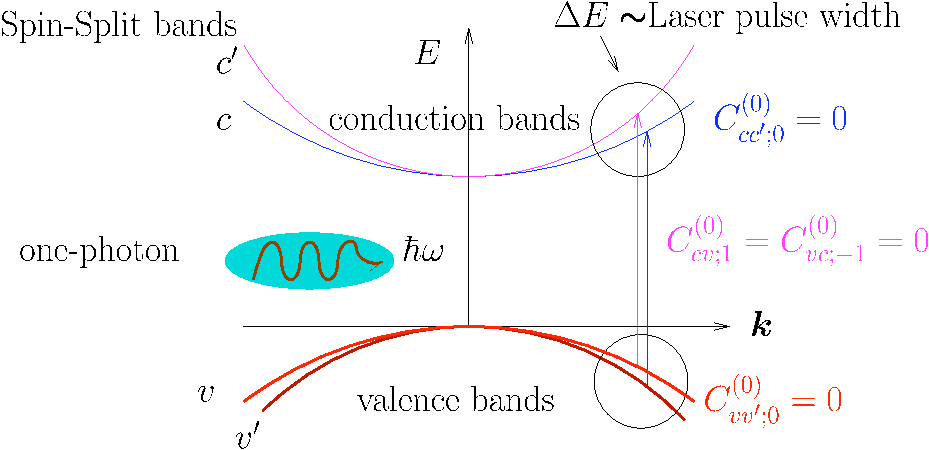
\includegraphics[width=10cm]{bands2-tmk}
\caption{(color online)
Coherence arise from simultaneous excitation of two close conduction bands, 
c and c', by the finite energy width of the laser beam. 
}
\label{fig:CoherenceBands}
\end{figure}


\subsection{Carrier injection rate $\dot n$}\label{sec:cir}
From Eq.~\eqref{trace3} we have that
\begin{eqnarray}\label{trace42}
\frac{d{\cal O}}{dt}
&=&
\frac{e^2}{i\hbar^2}
\int\frac{d^3k}{8\pi^3}
\sum_{vcc'}
{\cal O}_{c'c}r^a_{cv}r^b_{vc'}
\left(
\frac{1}{\omega-\omega_{c'v}-i\epsilon}
-
\frac{1}
{\omega-\omega_{cv}+i\epsilon}
\right)
E^a(\omega)E^{b\star}(\omega)
\\ \nonumber
&=&
\frac{e^2}{i\hbar^2}
\int\frac{d^3k}{8\pi^3}
\sum_{vcc'}
{\cal O}_{c'c}r^a_{vc'} r^b_{cv}
\left(
\frac{1}{\omega-\omega_{c'v}-i\epsilon}
-
\frac{1}
{\omega-\omega_{cv}+i\epsilon}
\right) 
E^{a\star}(\omega) E^b(\omega)
,
\end{eqnarray}  
where we only exchanged $a\leftrightarrow b$. Using Eq.~\eqref{eq:25}
\begin{eqnarray}\label{trace54}
\frac{d{\cal O}}{dt}
&=&
\frac{e^2}{i\hbar^2}
\int\frac{d^3k}{8\pi^3}
\sum_{vcc'}
{\cal O}_{c'c}r^a_{vc'} r^b_{cv}
\Big[
{\cal P}\left(
\frac{1}{\omega-\omega_{c'v}}
-
\frac{1}
{\omega-\omega_{cv}}
\right) 
\nonumber\\
&+&
i\pi\left(
\gd(\omega-\omega_{c'v})
+
\gd(\omega-\omega_{cv})
\right)
\Big]
E^a(-\omega) E^b(\omega)
\nonumber\\
&=&
\frac{e^2}{i\hbar^2}
\int\frac{d^3k}{8\pi^3}
\sum_{vcc'}
{\cal O}_{c'c}r^a_{vc'} r^b_{cv}
\Big[
{\cal P}\left(
\frac{\go_{c'c}}{(\omega-\omega_{c'v})
(\omega-\omega_{cv})}
\right) 
\nonumber\\
&+&
i\pi\left(
\gd(\omega-\omega_{c'v})
+
\gd(\omega-\omega_{cv})
\right)
\Big]
E^a(-\omega) E^b(\omega)
\nonumber\\
&\approx&
\frac{\pi e^2}{\hbar^2}
\int\frac{d^3k}{8\pi^3}
\sum_{vcc'}
{\cal O}_{c'c}r^a_{vc'} r^b_{cv}
\Big[
\gd(\omega-\omega_{c'v})
+
\gd(\omega-\omega_{cv})
\Big]
E^a(-\omega) E^b(\omega)
\nonumber\\
&=&
\frac{\pi e^2}{\hbar^2}
\int\frac{d^3k}{8\pi^3}
\sum_{vcc'}
\Big[
{\cal O}_{cc'}r^a_{vc} r^b_{c'v}
+
{\cal O}_{c'c}r^a_{vc'} r^b_{cv}
\Big]
\gd(\omega-\omega_{cv}) 
E^a(-\omega) E^b(\omega) 
.
\end{eqnarray}  
We take $\hat{\cal O}\to|\bfr\rangle\langle\bfr|$
 for the electron
number density, the
\begin{equation}\label{rho}
\hat{\cal O}_{cc'}=\langle c\bfk|\bfr\rangle\langle\bfr|c'\bfk\rangle
=\psi_{c\bfk}^*(\bfr) \psi_{c'\bfk}(\bfr)
\equiv\rho_{cc'}(\bfr;\bfk)
,
\end{equation}
the density matrix elements for the electron in the conduction bands $cc'$,
since we only want to calculate the DSP for electrons. 
Using time-invariance $\psi_{c(-\bfk)}(\bfr)=\psi_{c\bfk}^\star(\bfr)$
it follows that
$\rho_{cc'}(\bfr;-\bfk)=\rho_{c'c}(\bfr;\bfk)=\rho_{cc'}^\star(\bfr;\bfk)$. The
latter is the hermiticity of the density matrix.

Then,
the carrier injection rate is given by
\begin{eqnarray}\label{m1}
\dot n(\bfr)
&=&
\frac{\pi e^2}{\hbar^2}
\int\frac{d^3k}{8\pi^3}
\sum_{vcc'}
\Big[
\rho_{cc'}r^a_{vc} r^b_{c'v}
+
\rho_{c'c}r^a_{vc'} r^b_{cv}
\Big]
\gd(\omega-\omega_{cv}) 
E^a(-\omega) E^b(\omega)
,
\end{eqnarray} 
that we write as a response function, i.e.
\begin{equation}\label{rn}
\dot n(\bfr)=\xi^{ab}(\bfr;\go)   
E^a(-\omega) E^b(\omega)  
,
\end{equation}  
with
\begin{eqnarray}\label{xir}
\xi^{ab}(\bfr;\go)
&=&
\frac{\pi e^2}{\hbar^2}
\int\frac{d^3k}{8\pi^3}
\sum_{vcc'}
\Big[
\rho_{cc'}(\bfr;\bfk)   
r^a_{vc} 
(\bfk) 
r^b_{c'v}
(\bfk)
+
\rho_{c'c}(\bfr;\bfk)
r^a_{vc'} 
(\bfk) 
r^b_{cv}
(\bfk)
\Big]
\gd(\omega-\omega_{cv}(\bfk)
)
.
\end{eqnarray}  
To obtain the contribution from the $\ell$-th layer we simply do the
following integration
\begin{eqnarray}\label{xiz}
\xi^{ab}(\ell;\go)&=&\frac{1}{\gO}\int d\bfr {\cal F}_\ell(z)
\xi^{ab}(\bfr;\go)
\nonumber\\
&=&
\frac{\pi e^2}{\hbar^2}
\int\frac{d^3k}{8\pi^3}
\sum_{vcc'}
\Big[
\rho_{cc'}(\ell;\bfk)    
r^a_{vc} 
(\bfk)  
r^b_{c'v}
(\bfk)
+
\rho_{c'c}(\ell;\bfk) 
r^a_{vc'} 
(\bfk)  
r^b_{cv}
(\bfk)
\Big]
\gd(\omega-\omega_{cv}(\bfk)
)
\end{eqnarray}     
with
\begin{eqnarray}\label{rhoz1}
\rho_{cc'}(\ell;\bfk)&=&
\frac{1}{\gO}\int d\bfr\, {\cal F}_\ell(z)
\rho_{cc'}(\bfr;\bfk)
\nonumber\\
&=&
\frac{1}{\gO}\int d\bfr\, {\cal F}_\ell(z)
\psi_{c\bfk}^\star(\bfr)
\psi_{c'\bfk}(\bfr)
.
\end{eqnarray}  
For a bulk system (or the whole slab) we take ${\cal F}_\ell(z)=1$ and then
$\rho_{cc'}(\ell;\bfk)=\gd_{cc'}$, with which we get 
\begin{eqnarray}\label{xib}
\xi^{ab}(\go)  
&=&
\frac{2\pi e^2}{\hbar^2}
\int\frac{d^3k}{8\pi^3}
\sum_{vc} 
r^a_{vc}(\bfk) r^b_{cv}(\bfk)  
\gd(\omega_{cv}(\bfk)-\omega)  
,
\end{eqnarray}   
which is the same as Eq. (16) of Nastos et al. (PRB {\bf 76}, 205113
(2007)). We write Eq. (6) Mendoza et al. Physical Review B {\bf 74},
075318 (2006).􏰵
\begin{align}\label{imchi}
\mathrm{Im}[\chi^{ab}(\go)] 
&=
\frac{\pi e^2}{\hbar}
\int\frac{d^3k}{8\pi^3}
\sum_{vc}
r^a_{vc}(\bfk) r^b_{cv}(\bfk) 
\gd(\omega_{cv}(\bfk)-\omega) 
\nonumber\\
&=\frac{\hbar}{2}\xi^{ab}(\go).
\end{align}

Expanding the wave functions in plane waves we obtain
\begin{eqnarray}\label{rhoz}
\rho_{cc'}(\ell;\bfk)
&=&
\frac{1}{\gO}\int d\bfr\, {\cal F}_\ell(z)
\psi_{c\bfk}^*(\bfr)
\psi_{c'\bfk}(\bfr)
\nonumber\\
&=&
\sum_{\bfG,\bfG'} 
                          \left(
                                C^{\uparrow *}_{c\bfk}(\bfG),
                               C^{\downarrow *}_{c\bfk}(\bfG)
                                \right) 
                         \left(\begin{array}{c}
                                C^{\uparrow}_{c'\bfk}(\bfG')\\
                               C^{\downarrow}_{c'\bfk}(\bfG')\\
                                \end{array}\right) 
\frac{1}{\gO}\int d\bfr\, {\cal F}_\ell(z)
e^{i(\bfG-\bfG')\cdot\bfr}
\nonumber\\
&=&
\sum_{\bfG\bfG'}
\left(
C^{\uparrow *}_{c\bfk}(\bfG) C^{\uparrow}_{c'\bfk}(\bfG')
+
C^{\downarrow *}_{c\bfk}(\bfG) C^{\downarrow}_{c'\bfk}(\bfG') 
\right)
\delta_{\mathbf{G}_{\|},\mathbf{G}'_{\parallel}}
f_\ell(G_\perp - G^{\prime}_\perp),
\nonumber\\
.
\end{eqnarray} 
where the reciprocal lattice vectors $\mathbf{G}$ are decomposed
into components parallel to the surface $\mathbf{G}_\parallel$,
and perpendicular to the surface $G_\perp \hat{\mathbf{z}}$, so
that $\mathbf{G} = \mathbf{G}_\parallel + G_\perp \hat{\mathbf{z}}$,
and
\begin{equation} \label{four}
f_{\ell}(g) =\frac{1}{L} \int_{z_\ell-\Delta_\ell^b}^{z_\ell+\Delta_\ell^f}
e^{igz}\,dz.
\end{equation}
The double-summation over the $\mathbf{G}$-vectors can be
efficiently done by creating a pointer array to identify all the
plane-wave coefficients associated with the same
$\mathbf{G}_\parallel$. 
We take $z_\ell$ at the center of an atom that belongs to layer 
$\ell$, and thus Eq.~(\ref{rhoz}) give
the $\ell$-th atomic layer contribution to the carrier injection rate 
Note that if we take the 
cut function ${\cal F}_\ell(z)$ to be unity through the whole slab, 
then $f_{\ell}(g)=\delta_{g,0}$ and from Eq.~\eqref{rhoz} one 
would recover the  results for the whole slab. Then we need to code
Eq.~\eqref{rhoz} as matrix elements and
\begin{eqnarray}\label{xizm1}
\xi^{ab}(\ell;\go)&=&
\frac{2\pi e^2}{\hbar^2}
\int\frac{d^3k}{8\pi^3}
\sum_{vcc'}
\frac{1}{2}\Big[
\rho_{cc'}(\ell;\bfk)    
r^a_{vc} 
(\bfk)  
r^b_{c'v}
(\bfk)
+
\rho_{c'c}(\ell;\bfk) 
r^a_{vc'} 
(\bfk)  
r^b_{cv}
(\bfk)
\Big]
\gd(\omega-\omega_{cv}(\bfk)
)
\end{eqnarray}     
as a response. We have put a factor of 2 in the prefactor so that 
$(\hbar/2)\dot n$ is 
$(\hbar/2)\times (2\pi e^2)/\hbar^2=\pi e^2/\hbar$ which is the same
prefactor as that of Im$[\chi^{ab}]$. Therefore it is more convenient to
redefine $\xi^{ab}\to (\hbar/2)\xi^{ab}\to\tilde\xi^{ab}$,  
\begin{eqnarray}\label{xizm2}
\tilde\xi^{ab}(\ell;\go)&=&
\frac{\pi e^2}{\hbar}
\int\frac{d^3k}{8\pi^3}
\sum_{vcc'}
\frac{1}{2}\Big[
\rho_{cc'}(\ell;\bfk)     
r^a_{vc} 
(\bfk)   
r^b_{c'v}
(\bfk)
+
\rho_{c'c}(\ell;\bfk)  
r^a_{vc'} 
(\bfk)   
r^b_{cv}
(\bfk)
\Big]
\gd(\omega-\omega_{cv}(\bfk)
)
\end{eqnarray}      
We notice that $(\hbar/2)\xi^{ab}(\go)=\mathrm{Im}[\chi^{ab}(\go)]$, with
$\ge^{ab}(\go)=1+4\pi\chi^{ab}(\go)$, however 
$(\hbar/2)\xi^{ab}(\ell;\go)\neq\mathrm{Im}[\chi^{ab}(\ell;\go)]$

We split the integral in Eq.~\eqref{xizm2} into $\bfk>0$ and $\bfk<0$,
and take the term in parenthesis,
\begin{eqnarray}\label{p1}
\Big[
\rho_{cc'}(\ell;\bfk)   
r^a_{vc} 
(\bfk) 
r^b_{c'v}
(\bfk)
+
\rho_{c'c}(\ell;\bfk)
r^a_{vc'} 
(\bfk) 
r^b_{cv}
(\bfk)
\Big]_{\bfk>0}
&+&
\Big[
\rho_{cc'}(\ell;\bfk)   
r^a_{vc} 
(\bfk) 
r^b_{c'v}
(\bfk)
+
\rho_{c'c}(\ell;\bfk)
r^a_{vc'} 
(\bfk) 
r^b_{cv}
(\bfk)
\Big]_{\bfk<0}
\nonumber\\
\rho_{cc'}(\ell;\bfk)   
r^a_{vc} 
(\bfk) 
r^b_{c'v}
(\bfk)
+
\rho_{c'c}(\ell;\bfk)
r^a_{vc'} 
(\bfk) 
r^b_{cv}
(\bfk)
&+&
\rho_{c'c}(\ell;\bfk)   
r^a_{cv} 
(\bfk) 
r^b_{vc'}
(\bfk)
+
\rho_{cc'}(\ell;\bfk)
r^a_{c'v} 
(\bfk) 
r^b_{vc}
(\bfk)
\nonumber\\
2\mathrm{Re}\left[\rho_{cc'}(\ell;\bfk)   
r^a_{vc} 
(\bfk) 
r^b_{c'v}
(\bfk)
\right]
&+&
2\mathrm{Re}\left[
\rho_{c'c}(\ell;\bfk)
r^a_{vc'} 
(\bfk) 
r^b_{cv}
(\bfk)
\right]
\nonumber\\
2\mathrm{Re}\big[
\rho_{cc'}(\ell;\bfk)   
r^a_{vc} 
(\bfk) 
r^b_{c'v}
(\bfk)
&+&
\rho_{c'c}(\ell;\bfk)
r^a_{vc'} 
(\bfk) 
r^b_{cv}
(\bfk)
\big]
\nonumber
\end{eqnarray}    
Then,
\begin{eqnarray}\label{xizm3}
\tilde\xi^{ab}(\ell;\go)
&=&
\frac{\pi e^2}{\hbar}
\int_{\bfk>0}\frac{d^3k}{8\pi^3}
\sum_{vcc'}
\mathrm{Re}\Big[
\rho_{cc'}(\ell;\bfk)    
r^a_{vc} 
(\bfk)  
r^b_{c'v}
(\bfk)
+
\rho_{c'c}(\ell;\bfk) 
r^a_{vc'} 
(\bfk)  
r^b_{cv}
(\bfk)
\Big]
\gd(\omega-\omega_{cv}(\bfk)
)
\nonumber\\
&=&
\frac{\pi e^2}{\hbar}
\int\frac{d^3k}{8\pi^3}
\sum_{vcc'}
\frac{1}{2}\mathrm{Re}\Big[
\rho_{cc'}(\ell;\bfk)    
r^a_{vc} 
(\bfk)  
r^b_{c'v}
(\bfk)
+
\rho_{c'c}(\ell;\bfk) 
r^a_{vc'} 
(\bfk)  
r^b_{cv}
(\bfk)
\Big]
\gd(\omega-\omega_{cv}(\bfk)
)
\nonumber\\
&=&
\frac{\pi e^2}{\hbar}
\int\frac{d^3k}{8\pi^3}
\sum_{vcc'}
\frac{1}{2}\mathrm{Re}\Big[
\rho_{cc'}(\ell)    
r^a_{vc} 
r^b_{c'v}
+
\rho_{c'c}(\ell) 
r^a_{vc'} 
r^b_{cv}
\Big]
\gd(\omega-\omega_{cv})
.
\end{eqnarray}     
where the 1/2 comes from the unrestricted values of $\bfk$ in the
integration, and the argument of $\bfk$ is omitted.  
Above shows that $\tilde\xi^{ab}(\ell;\go)$ is a real quantity, as it must!

\subsubsection{Units}

We obtain that in the S.I. system of units 
Eq.~\eqref{rn}, leads to 
\begin{align}\label{rn.n1}
[\dot n]&=[\xi] [E]^2 
\nonumber\\
\frac{1}{sm^3}&=[\xi] \frac{V^2}{m^2}
\nonumber\\
\Rightarrow 
[\xi]&=\frac{1}{msV^2}
. 
\end{align}
It so happens that in Gaussian (cgs) units   (see Eq.~\eqref{imchi}) 
\begin{align}\label{rn.n2}
\xi^{\rma\rmb}&=\frac{2}{\hbar}
\mathrm{Im}[\chi^{\rma\rmb}]
\nonumber\\
\Rightarrow  
\xi^{\rma\rmb}_{\mathrm{S.I.}}&=2\frac{\ge_0}{\hbar}
\mathrm{Im}[\chi^{\rma\rmb}_{\mathrm{cgs}}]
,
\end{align}  
where $\mathrm{Im}[\chi^{\rma\rmb}_{\mathrm{cgs}}]$ is  
dimensionless. Therefore, the units are 
\begin{align}\label{rn.n3}
[\xi^{\rma\rmb}_{\mathrm{S.I.}}]&=\frac{[\ge_0]}{[\hbar]}
=\frac{F/m}{Js}=\frac{C/mV}{CVs}
=\frac{1}{msV^2}
,
\end{align} 
which agree with Eq.~\eqref{rn.n1}.
\subsection{Degree of Spin Polarization: DSP}\label{dsp}

The degree of spin polarization is defined as
\begin{equation}\label{dsp1}
{\cal D}^a=\frac{\dot S^a}{(\hbar/2)\dot n}
.  
\end{equation}   
The prefactor of $(\hbar/2)\dot n$ is 
$(\hbar/2)\times (2\pi e^2)/\hbar^2=\pi e^2/\hbar$ which is the same
as that of Im$[\chi^{ab}]$. Therefore it is more convenient to
redefine 
$\dot{\tilde n}=(\hbar/2)\dot n=\tilde\xi^{ab}E^a(-\go)E^b(\go)$,  
and
\begin{equation}\label{dsp2}
{\cal D}^a=\frac{\dot S^a}{\dot{\tilde n}}
.
\end{equation}
The prefactor of $\dot S^2$ is
 $(\pi e^2/\hbar^2)\times(\hbar/2)\propto \pi e^2/\hbar$
where $\hbar/2$ comes from the units of the spin matrix elements that
are given through $\hat S^a=(\hbar/2)\hat\sigma^a$. Therefore we see
that ${\cal D}^a$ is a dimensionless quantity.

In the code subroutine \verb=inparams.f90= we use the prefactor 
of Im$[\chi^{ab}]$ (\verb=Chi1_factor=) as the prefactor of
$\tilde\xi^{ab}$, although we don't call it ``tilde'', indeed we call
it \verb=ndotccp=  for the conduction.

In general, for a circularly polarized beam of light propagating along
$z$ (which is normal to the surface), the DSP is equal to
\begin{equation}\label{dsp3}
{\cal D}^z=\frac{2\zeta^{zxy}}{\tilde\xi^{xx}+\tilde\xi^{yy}}
,
\end{equation} 
where $\zeta^{zxy}$ is taken as it comes from the code!
(see Eq.~\eqref{sdotnew} and recall that $\tilde\zeta^{abc}=i\zeta^{abc}$)

\section{Electrical Current} 

The operator of the electrical current is given by,
\begin{align}\label{ec.1}
\hat\bfJ=\frac{1}{\gO}e\hat\bfv
.
\end{align}
From Eq.~\eqref{trace54}
\begin{align}\label{ec.2}
\dot J^\rma  
&=
\frac{\pi e^3}{\hbar^2}
\int\frac{d^3k}{8\pi^3}
\sum_{vcc'}
\Big[ 
v^\rma_{cc'}r^\rmb_{vc} r^\rmc_{c'v}
+ 
v^\rma_{c'c}r^\rmb_{vc'} r^\rmc_{cv}
\Big]
\gd(\omega-\omega_{cv})  
E^\rmb(-\omega) E^\rmc(\omega) 
\nonumber\\
&=
\eta^{\rma\rmb\rmc} 
E^\rmb(-\omega) E^\rmc(\omega) 
,
\end{align} 
where the volume factor, $\gO$, is included implicitly, and
\begin{align}\label{ec.3}
\eta^{\rma\rmb\rmc} 
&=
\frac{\pi e^3}{\hbar^2}
\int\frac{d^3k}{8\pi^3}
\sum_{vcc'}
\Big[ 
v^\rma_{cc'}(\bfk) r^\rmb_{vc}(\bfk) r^\rmc_{c'v}(\bfk) 
+
v^\rma_{c'c}(\bfk) r^\rmb_{vc'}(\bfk) r^\rmc_{cv}(\bfk) 
\Big]
\gd(\omega-\omega_{cv}(\bfk)) 
\nonumber\\
&=
\frac{\pi e^3}{\hbar^2}
\int\frac{d^3k}{8\pi^3}
\sum_{vcc'}
\Big[ 
\Big(v^\rma_{cc'}(\bfk) r^\rmb_{vc}(\bfk) r^\rmc_{c'v}(\bfk) \Big)\Big|_{\bfk>0} 
+
\Big(v^\rma_{cc'}(\bfk) r^\rmb_{vc}(\bfk) r^\rmc_{c'v}(\bfk)\Big)\Big|_{\bfk<0} 
\nonumber\\
&+
\Big(v^\rma_{c'c}(\bfk) r^\rmb_{vc'}(\bfk) r^\rmc_{cv}(\bfk)\Big)\Big|_{\bfk>0} 
+
\Big(v^\rma_{c'c}(\bfk) r^\rmb_{vc'}(\bfk) r^\rmc_{cv}(\bfk)\Big)\Big|_{\bfk<0} 
\Big]
\gd(\omega-\omega_{cv}(\bfk)) 
\nonumber\\
&=
\frac{\pi e^3}{\hbar^2}
\int_{\bfk>0}
\frac{d^3k}{8\pi^3}
\sum_{vcc'}
\Big[ 
v^\rma_{cc'}(\bfk) r^\rmb_{vc}(\bfk) r^\rmc_{c'v}(\bfk) 
-
v^\rma_{c'c}(\bfk) r^\rmb_{cv}(\bfk) r^\rmc_{vc'}(\bfk) 
\nonumber\\
&+
v^\rma_{c'c}(\bfk) r^\rmb_{vc'}(\bfk) r^\rmc_{cv}(\bfk) 
-
v^\rma_{cc'}(\bfk) r^\rmb_{c'v}(\bfk) r^\rmc_{vc}(\bfk) 
\Big]
\gd(\omega-\omega_{cv}(\bfk)) 
\nonumber\\
&=
\frac{\pi e^3}{\hbar^2}
\frac{1}{2}
\int
\frac{d^3k}{8\pi^3}
\sum_{vcc'}
\Big[ 
v^\rma_{cc'}(\bfk) r^\rmb_{vc}(\bfk) r^\rmc_{c'v}(\bfk) 
-
(v^\rma_{cc'}(\bfk) r^\rmb_{vc}(\bfk) r^\rmc_{c'v}(\bfk))^*
\nonumber\\
&+
v^\rma_{c'c}(\bfk) r^\rmb_{vc'}(\bfk) r^\rmc_{cv}(\bfk) 
-
(v^\rma_{c'c}(\bfk) r^\rmb_{vc'}(\bfk) r^\rmc_{cv}(\bfk) )^*
\Big]
\gd(\omega-\omega_{cv}(\bfk)) 
\nonumber\\
&=
\frac{i\pi e^3}{\hbar^2}
\int\frac{d^3k}{8\pi^3}
\sum_{vcc'}
\mathrm{Im}\Big[ 
v^\rma_{cc'}(\bfk) r^\rmb_{vc}(\bfk) r^\rmc_{c'v}(\bfk) 
+
v^\rma_{c'c}(\bfk) r^\rmb_{vc'}(\bfk) r^\rmc_{cv}(\bfk) 
\Big]
\gd(\omega-\omega_{cv}(\bfk)) 
,
\end{align}
 since $\bfv_{nm}(-\bfk)=-\bfv_{mn}(\bfk)$ and 
$\bfr_{nm}(-\bfk)=\bfr_{mn}(\bfk)$.

\subsection{Units}

We obtain that in the S.I. system of units 
Eq.~\eqref{ec.2}, leads to ($J=CV$) 
\begin{align}\label{ec.4}
[\dot J]&=[\eta] [E]^2 
\nonumber\\
\frac{1}{s}\frac{1}{m^3} C\frac{m}{s}
&=[\eta] \frac{V^2}{m^2}
\nonumber\\
\Rightarrow 
[\eta]&=\frac{C}{s^2V^2}=\frac{C^3}{J^2s^2}
,
\end{align}
which are the same units as those of the injection
current.\cite{cabellosPRB11}

\subsection{Swarm Velocity} 

We define the swarm velocity as  
\begin{align}\label{sv.1}  
v^\rma_s&=\frac{\dot J^\rma}{e\dot n}
\nonumber\\
&=\frac{\eta^{\rma\rmb\rmc}E^\rmb(-\go)E^\rmc(\omega)}
{e\xi^{\rmb\rmc}E^\rmb(-\go)E^\rmc(\omega)}
\nonumber\\
\Rightarrow[v_s]&=\frac{[\eta]}{C[\xi]}=\frac{\frac{C^3}{J^2s^2}}{\frac{C}{msV^2}}
=\frac{mC^2V^2}{sJ^2}=\frac{m}{s}
,
\end{align}  
where we used Eq.~\eqref{ec.4} and \eqref{rn.n3}.
Now, since 
$\eta^{\rma\rmb\rmc}
=-\eta^{\rma\rmc\rmb}$, $\eta^{\rma\rmb\rmb}=0$, and then
\begin{align}\label{sv.2}
\dot J^\rma
&=\eta^{\rma\rmb\rmc}E^\rmb(-\go)E^\rmc(\omega) 
\nonumber\\
&=\eta^{\rma\rmb\rmc}E^\rmb(-\go)E^\rmc(\omega) 
+
\eta^{\rma\rmc\rmb}E^\rmc(-\go)E^\rmb(\omega) \quad 
\quad(\rmb\neq\rmc) 
\nonumber\\
&=\eta^{\rma\rmb\rmc}\Big(E^{\rmb *}(\go)E^\rmc(\omega) 
-
E^{\rmc *}(\go)E^\rmb(\omega)\Big) 
=\eta^{\rma\rmb\rmc}\Big(E^{\rmb *}(\go)E^\rmc(\omega) 
-
(E^{\rmb *}(\go)E^\rmc(\omega))^*\Big) 
\quad(\rmb\neq\rmc) 
\nonumber\\
&=-2i\eta^{\rma\rmb\rmc}\mathrm{Im}\Big[E^{\rmb}(\go)E^{\rmc *}(\omega) \Big]
\quad(\rmb\neq\rmc) 
,
\end{align}
and since $\eta^{\rma\rmb\rmc}$ has an $i$, above is a real quantity,
as it should. Now, from above the electric field must have a component
along b and c, then
\begin{align}\label{sv.3}
\dot n
&=\xi^{ij}E^i(-\go)E^j(\omega) 
\nonumber\\
&=
\xi^{\rmb\rmb}|E^\rmb(\go)|^2 +\xi^{\rmc\rmc}|E^\rmc(\go)|^2 
+2 \xi^{\rma\rmb}E^\rmb(-\go)E^\rmc(\omega) 
\quad(\rmb\neq\rmc) 
,
\end{align}
since $\xi^{ij}=\xi^{ji}$, and in going to principal axis $\xi^{ij}=0$
for $i\neq j$. Finally,
\begin{align}\label{sv.4}  
v^\rma_s&=
\frac  
{-2i\eta^{\rma\rmb\rmc}\sin(\phi_\rmb-\phi_\rmc)}
{\xi^{\rmb\rmb} +\xi^{\rmc\rmc}}
,
\end{align}  
where $E^\rma(\go)=\bfE_0e^{i\phi_\rma}$, and the maximum swarm
velocity is
\begin{align}\label{sv.4} 
v^\rma_{s,max}&=
\frac 
{2\tilde\eta^{\rma\rmb\rmc}}
{\xi^{\rmb\rmb} +\xi^{\rmc\rmc}}
,
\end{align} 
with $\tilde\eta^{\rma\rmb\rmc}=i\eta^{\rma\rmb\rmc}$.
%%%%%%%%
\section{Time Reversal}\label{sec:tr}
In classical mechanics,
\begin{align}\label{e.6}
\bfp=m\frac{d\bfr}{dt}\Big|_{t\to -t}\to -\bfp 
,
\end{align} 
and
$\bfr(t)=\bfr(-t)$, 
therefore if $\bfr(t),\bfp(t)$ is a solution of Newton's equations of motion, so 
is $\bfr(-t),-\bfp(-t)$, therefore the Hamiltonian satisfies
\begin{align}\label{e.7}  
H(\bfr,\bfp)&=H(\bfr,-\bfp) 
,
\end{align}  
from which $H$ is an even function of $\bfp$.

In quantum mechanics,
\begin{align}\label{e.8}
\hat\bfp &=-i\hbar\bfgnabla 
\nonumber\\
\Rightarrow \hat\bfp^* &=-\hat\bfp,
\end{align}
where we se that the complex conjugation is equivalent to 
time-reversal, therefore we define the operator of complex conjugation, $\hat K_0$, as 
\begin{align}\label{e.9}
\hat K_0\Big(-i\hbar\bfgnabla\Big)K^{-1}_0=i\hbar\bfgnabla  
,
\end{align}  
in the space representation. $\hat K_0$ is the Wigner's time-reversal 
operator, that satisfies
\begin{align}\label{e.12}
\hat K^2_0=1  
,
\end{align} 
since applying complex conjugation twice give back the original
result, and then 
\begin{align}\label{e.13}
\hat K^{-1}_0=\hat K_0 
,
\end{align}
is the inverse operator, with which Eq.~\eqref{e.12} is satisfied.
Eq.~\eqref{e.7} becomes
\begin{align}\label{e.10} 
\hat H_0(\bfr,-i\hbar\bfgnabla )&=\hat H_0(\bfr,i\hbar\bfgnabla ) 
,
\end{align} 
which, in space representation, $\hat H_0$ is a real function. 
We rewrite Eq.~\eqref{e.14} as,
\begin{align}\label{e.11}
\hat K_0\hat\bfp \hat K^{-1}_0&=-\hat\bfp 
\nonumber\\
\hat K_0\hat\bfp 
&=-\hat\bfp \hat K_0  
,
\end{align}  
whit which we obtain that
\begin{align}\label{e.11n}
\hat K_0\hat\bfp^2
&=
\hat K_0 
\hat\bfp\cdot \hat\bfp
=-\hat\bfp\cdot \hat K_0 \hat\bfp
=\hat\bfp\cdot \hat\bfp\hat K_0 
=\hat p^2\hat K_0 
.
\end{align} 
The following Hamiltonian gives that 
\begin{align}\label{e.20}
\hat H_0&=\frac{\hat p^2}{2m}+V(\bfr) 
\nonumber\\
\hat K_0 
\hat H_0&=\hat K_0 \frac{\hat p^2}{2m}+\hat K_0  V(\bfr) 
\nonumber\\
&=
\Big( \frac{\hat p^2}{2m}+  V(\bfr)\Big) \hat  K _0 
=\hat H_0\hat K_0,
\nonumber\\
&\Rightarrow [\hat H_0,\hat K_0]=0,
\nonumber\\
&\Rightarrow \hat K_0\hat H_0\hat K^{-1}_0=\hat H_0,
\end{align}
assuming that $V(\bfr)$ is real. Therefore we obtain that
\begin{align}\label{e.13n}
\hat K_0\Big(\hat H_0\psi&=E\psi\Big) 
\nonumber\\
\hat H_0 \Big(\hat K_0\psi\Big)&=E \Big(\hat K_0\psi\Big)  
,
\end{align} 
from where we see that $\psi$ and $\hat K_0\psi$ are degenerate, as
the have the same energy $E$. Also,
\begin{align}\label{e.14}
\Big(\hat H_0\psi&=E\psi\Big)^* 
\nonumber\\
\hat H_0 \psi^*&=E \psi^* 
,
\end{align}
from where
we have that
\begin{align}\label{e.11nn}
\hat K_0\psi(\bfr)=\psi^*(\bfr)
.
\end{align}

In the presence of spin, the hamiltonian is given by 
\begin{align}\label{e.30}
\hat H&=
\frac{\hat p^2}{2m} + V(\bfr) 
+\frac{\hbar^2}{4m^2c^2}
\hat\bfgs\cdot(\bfgnabla V(\bfr)\times\hat \bfp) 
\nonumber\\
&=
\hat H_0+
\hat\bfgs\cdot(\calbv (\bfr)\times\hat \bfp) 
,
\end{align} 
where $\hat H_0=\frac{\hat p^2}{2m} + V(\bfr) $ is already treated
above, and $\calbv(\bfr)=\frac{\hbar^2}{4m^2c^2}\bfgnabla V (\bfr)$.
Now, we define a time-reversal operator $\hat K$ that leaves above
hamiltonian invariant, then 
\begin{align}\label{e.31}
\hat H 
=
\hat K 
\hat H 
\hat K^{-1}
&=
\hat K 
\hat H_0 
\hat K^{-1}
+
\hat K 
\hat\bfgs\cdot(\calbv (\bfr)\times\hat \bfp) \hat K^{-1}
\nonumber\\
&=
\hat K \hat H_0 \hat K^{-1}
+
\hat K \hat\bfgs \hat K^{-1}
\cdot(
\hat K \calbv (\bfr) \hat K^{-1}
\times 
\hat K \hat \bfp \hat K^{-1}
).
\end{align}
From Eq.~\eqref{e.11} and the fact that functions of $\bfr$ are
invariant under time-reversal, we propose that
\begin{align}\label{e.32}
\hat K \hat \bfp \hat K^{-1}&=-\hat\bfp,
\nonumber\\
\hat K \hat H_0 \hat K^{-1}&=H_0
\nonumber\\
\hat K \calbv (\bfr) \hat K^{-1}&=\calbv (\bfr)
\end{align}
and thus,
\begin{align}\label{e.33}
\hat K \hat\bfgs \hat K^{-1}&=-\hat\bfgs 
,
\end{align}
to keep $\hat H$ invariant. Again, $[\hat H,\hat K]=0$, and $\psi$ is
degenerate with $\hat K\psi$.

We write $\hat K=\hat U \hat K_0$ and look for $\hat U$.
From Eq.~\eqref{eq:pauliMatrix}
\begin{align}\label{e.34}
\hat
\gs^*_x=\hat\gs_x 
\quad 
\hat\gs^*_y=-\hat\gs_y 
\quad 
\hat\gs^*_z=\hat\gs_z
,
\end{align}
and using $\hat\gs_i\hat\gs_j=i\ge_{ijk}\hat\gs_k$ and
$\{\hat\gs_i,\hat\gs_j\}=0$, we can show that
\begin{align}\label{e.34n}
\hat\gs_y\bfgs^*=
(\hat\gs_y\hat\gs_x,-\hat\gs_y\hat\gs_y,\hat\gs_y\hat\gs_z)
&=-(\hat\gs_x,\hat\gs_x,\hat\gs_x)\gs_y
=-\hat\bfgs\hat\gs_y
\nonumber\\
\Rightarrow 
\hat\gs_y\bfgs^*\hat\gs^{-1}_y&=-\hat\bfgs 
\nonumber\\
\Rightarrow 
\hat\gs_y\hat K_0\bfgs\hat K_0^{-1}\hat\gs^{-1}_y&=-\hat\bfgs 
\nonumber\\
\Rightarrow 
\hat K&=\hat\gs_y\hat K_0
.
\end{align}
since $\hat K_0\hat\bfgs\hat K^{-1}_0=\hat\bfgs^*$ 
Now, we confirm that $\hat K=\hat\gs_y\hat K_0$ really works, then we take
\begin{align}\label{e.35}
\hat H_{so}=
\frac{\hbar^2}{4m^2c^2}
\hat\bfgs\cdot (\bfgnabla V(\bfr)\times\hat \bfp) 
\neq \hat H^*_{so}
,
\end{align}
since $\hat \bfp^*=-\hat\bfp$ but $\bfgs^*\neq\bfgs$,
and write 
$\hat H_{so}=
\hat\bfgs\cdot \hat\bfA $
with 
$\hat\bfA=\frac{\hbar^2}{4m^2c^2}(\bfgnabla V(\bfr)\times\hat \bfp)$, 
and obtain that
\begin{align}\label{e.36}
\hat H_{so}&=\hat A_x \hat \gs_x +\hat A_y \hat \gs_y +\hat A_z \hat \gs_z 
\nonumber\\
\hat H^*_{so}&=-\hat A_x \hat \gs_x +\hat A_y \hat \gs_y -\hat A_z \hat \gs_z 
\nonumber\\
\hat\gs_x\hat H^*_{so}&=\Big(-\hat A_x \hat \gs_x -\hat A_y \hat \gs_y +\hat A_z \hat \gs_z\Big)\hat\gs_x 
\nonumber\\
\hat\gs_z\hat H^*_{so}&=\Big(\hat A_x \hat \gs_x -\hat A_y \hat \gs_y -\hat A_z \hat \gs_z\Big)\hat\gs_z 
\nonumber\\
\hat\gs_y\hat H^*_{so}&=\hat H_{so}\hat\gs_y 
\nonumber\\
\Rightarrow \hat\gs_y\hat H^*_{so}\hat\gs^{-1}_y&=\hat H_{so}
\nonumber\\
\Rightarrow \hat\gs_y\hat K_0\hat H_{so}\hat K^{-1}_0\hat\gs^{-1}_y&=\hat H_{so}
\nonumber\\
\Rightarrow \hat K\hat H_{so}\hat K^{-1}&=\hat H_{so}
,
\end{align} 
where we see that  $\hat U=\hat\gs_y$ works and that $\hat
U=i\hat\gs_y$ will work as well.

\subsection{Bloch's theorem}

We define $T_{\bfR_\ell}$ as the translation operator, such that,
\begin{align}\label{ee.1} 
T_{\bfR_\ell}f(\bfr)=f(\bfr+\bfR_\ell)  
,
\end{align} 
for a crystal,
\begin{align}\label{ee.2} 
T_{\bfR_\ell}H(\bfr)=H(\bfr+\bfR_\ell) =H(\bfr) 
,
\end{align} 
then
\begin{align}\label{ee.2n}
T_{\bfR_\ell}\Big(H\psi(\bfr)&=E\psi(\bfr)\Big) 
\nonumber\\ 
H \Big(T_{\bfR_\ell}\psi(\bfr)\Big)&=E \Big(T_{\bfR_\ell}\psi(\bfr)\Big) 
\nonumber\\
\Rightarrow \psi(\bfr)&=e^{i\phi}T_{\bfR_\ell}\psi(\bfr)
,
\end{align}
from
\begin{align}\label{ee.3}
|\psi(\bfr)|^2=|T_{\bfR_\ell}\psi(\bfr)|^2
\nonumber\\
\Rightarrow T_{\bfR_\ell}
\psi(\bfr)=e^{i\ga^{\strut}_\ell}
\psi(\bfr)
,
\end{align}
where $\bfR_\ell$ 
are the crystal lattice vectors, that satisfy 
$\bfR_\ell+\bfR_m=\bfR_p$ or
$T_{\bfR_\ell}T_{\bfR_m}=T_{\bfR_p}$. 
This last requirement is easily satisfied by
$\mathrm{Exp}[i(\ga^{\strut}_\ell
+\ga^{\strut}_m)]=\mathrm{Exp}[i\ga^{\strut}_p]$, where we take
$\ga^{\strut}_\ell=\bfk\cdot\bfR_\ell$, 
and finally get that
\begin{align}\label{ee.4} 
T_{\bfR_\ell}\psi(\bfr)=e^{i \bfk\cdot\bfR_\ell}\psi(\bfr)  
,
\end{align}    
where $\bfk$ is used to classify the states (then, its the crystal
momentum), so Bloch's Theorem reads,
\begin{align}\label{ee.5} 
T_{\bfR_\ell}\psi_n(\bfk,\bfr)=e^{i \bfk\cdot\bfR_\ell}\psi_n(\bfk,\bfr) 
,
\end{align}    
where $n$ is the energy band. The Bloch's wave function is written as
\begin{align}\label{ee.6}
\psi_n(\bfk,\bfr)&=e^{i \bfk\cdot\bfr}u_n(\bfk,\bfr)  
\nonumber\\ 
\Rightarrow T_{\bfR_\ell}\psi_n(\bfk,\bfr)&=\psi_n(\bfk,\bfr+\bfR_\ell)  
= 
e^{i \bfk\cdot(\bfr+\bfR_\ell)}u_n(\bfk,\bfr+\bfR_\ell) 
= 
e^{i \bfk\cdot\bfR_\ell}   
e^{i \bfk\cdot\bfr}  
u_n(\bfk,\bfr) 
\nonumber\\
&=e^{i \bfk\cdot\bfR_\ell} 
\psi_n(\bfk,\bfr)  
,
\end{align}    
since $u_n(\bfk,\bfr+\bfR_\ell) =u_n(\bfk,\bfr) $ is periodic, thus
fulfilling Bloch's theorem. The reciprocal lattice vectors, $\bfG$ are
defined, by (we drop the labels in $\bfG$ and $\bfR$, for ease of notation)
\begin{align}\label{ee.7}
e^{i\bfG\cdot\bfR}=1
,
\end{align} 
 thus we have that
\begin{align}\label{ee.8}
\Rightarrow T_{\bfR}\psi_n(\bfk+\bfG,\bfr)&= 
e^{i (\bfk+\bfG)\cdot\bfR}\psi_n(\bfk+\bfG,\bfr) 
= 
e^{i \bfk\cdot\bfR}\psi_n(\bfk+\bfG,\bfr) 
,
\end{align}    
which has the same eigenvalue as 
Eq.~\eqref{ee.5}, then
\begin{align}\label{ee.9}
\psi_n(\bfk+\bfG,\bfr) =\psi_n(\bfk,\bfr) 
,
\end{align}
is periodic in reciprocal space as well. 
From Eq.~\eqref{ee.5}, it also follows that
\begin{align}\label{ee.10}
T_{\bfR}\psi^*_n(\bfk,\bfr)&=
e^{-i \bfk\cdot\bfR}\psi^*_n(\bfk,\bfr) 
\nonumber\\ 
T_{\bfR}\psi_n(-\bfk,\bfr)&=
e^{-i \bfk\cdot\bfR}\psi_n(-\bfk,\bfr) 
\nonumber\\
\Rightarrow \psi_n(-\bfk,\bfr)&=\psi^*_n(\bfk,\bfr)
\nonumber\\
\Rightarrow e^{i(-\bfk)\cdot\bfr}u_n(-\bfk,\bfr) 
&=  
e^{-i\bfk\cdot\bfr}u^*_n(\bfk,\bfr) 
\nonumber\\
\Rightarrow u_n(-\bfk,\bfr) 
&=  
u^*_n(\bfk,\bfr) 
,
\end{align}   
thus complex-conjugation is equivalente to taking $\bfk\to
-\bfk$. Then,
 \begin{align}\label{e.n11}
\Big(
H\psi_n(\bfk,\bfr)&=E_n(\bfk)\psi_n(\bfk,\bfr) 
\Big)^*
\nonumber \\ 
H\psi^*_n(\bfk,\bfr)&=E_n(\bfk)\psi^*_n(\bfk,\bfr) 
\nonumber \\
H\psi_n(-\bfk,\bfr)&=E_n(\bfk)\psi_n(-\bfk,\bfr) 
\nonumber \\ 
\bfk &\to -\bfk
\nonumber \\  
H\psi_n(\bfk,\bfr)&=E_n(-\bfk)\psi_n(\bfk,\bfr) 
\nonumber \\ 
\Rightarrow
E_n(\bfk)&=E_n(-\bfk)
,
\end{align}

\subsection{Spin-Orbit coupling}

Schr\"odinger equation with the spin-orbit coupling reads 
\begin{align}\label{e.5}
\Big[\frac{\hat p^2}{2m} + V(\bfr) 
+\frac{\hbar^2}{4m^2c^2}\hat\bfgs\cdot(\bfgnabla V(\bfr)\times\hat \bfp) 
\Big]\psi(\bfr,s)=E\psi(\bfr,s) 
,
\end{align} 
which is invariant upon time reversal, $t\to -t$. 
The Bloch states when the $H_{so}$ is present, are spinors of the form
\begin{eqnarray}\label{e.37n}
\psi=\left(\begin{array}{c}     
u  \\     
v  
\end{array}\right)     
\end{eqnarray}     
and Eq.~\eqref{e.5} reduces to
\begin{eqnarray}\label{e.37nn}
\left(\begin{array}{cc}    
H_0+A_z & A_x-iA_y  \\    
A_x+iA_y & H_0-A_z  \\    
\end{array}\right)     
\left(\begin{array}{c}     
u  \\     
v  
\end{array}\right)     
=
E
\left(\begin{array}{c}     
u  \\     
v  
\end{array}\right)     
\end{eqnarray}    
where in general $u\neq v\neq 0$, and
$|u|^2$ is the probability of spin up,  
while
$|v|^2$ is the probability of spin down. Then, we can write 
\begin{eqnarray}\label{e.38}
\braket{\bfr}{ns\bfk}=\psi_{ns}(\bfk;\bfr)
=\left(\begin{array}{c}    
u_{n s}(\bfk;\bfr)  \\    
v_{n s}(\bfk;\bfr)  
\end{array}\right)     
e^{i\bfk\cdot\bfr}
=\left(\begin{array}{c}    
u_{n s}(\bfk;\bfr;\uparrow)  \\    
v_{n s}(\bfk;\bfr;\downarrow)  
\end{array}\right)     
e^{i\bfk\cdot\bfr}
\end{eqnarray}    
where $n$ denotes the band and $s$ the spin.
%, where $\bar s$ is the spin opposite to $s$.

We would like to express the matrix elements of an operator upon applying
time-reversal symmetry, and relate them to those before applying
time-reversal.
To this end, we first prove the following identity of the  scalar
product between to spinor wavefunctions with and without time-reversal,
\begin{align}\label{z.1}
(\hat K\phi,\hat K\psi)=(\psi,\phi)  
.  
\end{align}   
On one hand,
\begin{align}\label{z.2}
(\psi,\phi)&
=\int dx\, \psi^\dagger\phi 
\nonumber\\
&=\int dx\, (\psi^*_1,\psi^*_2)  
\left(\begin{array}{c} 
\phi_1\\
\phi_2  
\end{array}\right)  
=
\int dx\, (\psi^*_1\phi_1+\psi^*_2\phi_2)  
. 
\end{align}  
On the other hand, we first realize that
\begin{eqnarray}\label{z.3}
\hat K\phi
&=i\hat\gs_y\hat K_0\phi=
\left(\begin{array}{cc}  
0  & 1 \\  
-1 & 0  
\end{array}\right)  
\left(\begin{array}{c}  
\phi^*_1\\
\phi^*_2
\end{array}\right)   
\nonumber\\
&=
\left(\begin{array}{c} 
\phi^*_2\\
-\phi^*_1
\end{array}\right)  
, 
\end{eqnarray} 
where we used Eq.~\eqref{eq:pauliMatrix}.
Then,  
\begin{align}\label{z.4}
(\hat K\phi,\hat K\psi)&
=\int dx\, (\hat K\phi)^\dagger\hat K\psi 
\nonumber\\
&=\int dx\, (\phi_2,-\phi_1) 
\left(\begin{array}{c} 
\psi^*_2\\
-\psi^*_1 
\end{array}\right)  
=
\int dx\, (\phi_2\psi^*_2+\phi_1\psi^*_1) 
 \quad\mathrm{Q.E.D.}
\end{align} 
Now, we denote $\hat K \psi=\tilde\psi$, so Eq.~\eqref{z.1} can be
written as,
\begin{align}\label{z.5}
(\hat K\phi,\hat K\psi)=(\tilde\phi,\tilde\psi)  =(\psi,\phi)  
,
\end{align}  
but since the dot product also satisfies $(\psi,\phi) =(\phi,\psi)^*$,
in braket notation we obtain this useful relationship, 
\begin{align}\label{z.6a}
\braket{\tilde\phi}{\tilde\psi}
=
\braket{\psi}{\phi}
=
\braket{\phi}{\psi}^*
.  
\end{align} 
For an operator $\hat\calo$ 
for which, 
$\hat\calo\ket{\phi}=\ket{\varphi}$, ww obtain the following identity,
\begin{align}\label{z.6}
\bra{\psi}\hat\calo\ket{\phi}
&=
\braket{\psi}{\varphi}
=
\braket{\tilde\varphi}{\tilde\psi}
=
\braket {\tilde\psi}{\tilde\varphi}^*
\nonumber\\
&
=
\bra{\tilde\psi}\hat K\ket{\varphi}^*
=
\bra{\tilde\psi}\hat K\hat\calo\ket{\phi}^*
=
\bra{\tilde\psi}\hat K\hat\calo\hat K^{-1}\hat K\ket{\phi}^*
\nonumber\\
&=
\bra{\tilde\psi}\hat K\hat\calo\hat K^{-1}\ket{\tilde\phi}^* 
=
\bra{\tilde\phi}\hat K\hat\calo\hat K^{-1}\ket{\tilde\psi}
\nonumber\\
\mathrm{or}\quad 
\bra{\tilde\psi}\hat K\hat\calo\hat K^{-1}\ket{\tilde\phi}^* 
&=
\bra{\psi}\hat\calo\ket{\phi}
\nonumber\\
\pm\bra{\tilde\psi}\hat\calo\ket{\tilde\phi}^* 
&=
\bra{\psi}\hat\calo\ket{\phi}
\nonumber\\
\bra{\tilde\psi}\hat\calo\ket{\tilde\phi}^* 
&=
\pm\bra{\psi}\hat\calo\ket{\phi}
. 
\end{align}
 


Now, from 
Eqs.~\eqref{eq:pauliMatrix}, \eqref{ee.10} 
and ~\eqref{e.38}
\begin{align}\label{e.40}
i\hat\gs_y\hat K_0
\ket{ns;\bfk}
&=
i\hat\gs_y\ket{ns;-\bfk}
,
\end{align}  
and
\begin{eqnarray}\label{e.38nnn}
i\hat\gs_y\ket{ns;-\bfk}
&\to  
\left(\begin{array}{cc}   
0  & 1 \\   
-1 & 0  
\end{array}\right)  
\left(\begin{array}{c}   
u_{n s}(-\bfk;\bfr)  \\   
v_{n s}(-\bfk;\bfr)  
\end{array}\right)    
e^{-i\bfk\cdot\bfr}
\nonumber\\
&=
\left(\begin{array}{c} 
v_{ns}(-\bfk;\bfr)  \\ 
-u_{ns}(-\bfk;\bfr)  
\end{array}\right)   
e^{-i\bfk\cdot\bfr}
\equiv \braket{\bfr}{n\bar s;-\bfk}
.  
\end{eqnarray}  
We see that if 
$|u_{ns}(\bfk;\bfr)|^2>|v_{ns}(\bfk;\bfr)|^2$  
is true for 
$\braket{\bfr}{ns;\bfk}$, 
meaning ``spin-up'' like, 
then the fact that in
$\braket{\bfr}{n\bar s;-\bfk}$ 
$|u_{ns}(\bfk;\bfr)|^2$ and $|v_{ns}(\bfk;\bfr)|^2$ are reversed in
the entries of the spinor, would mean that  
$\braket{\bfr}{n\bar s;-\bfk}$ 
is ``spin-down'' like. Therefore, $\bar s$ is used to denote this
fact, and in summary, 
\begin{align}\label{e.40nnnn}
\hat K\ket{ns;\bfk}=
&
=e^{i\phi_n}\ket{n\bar s;-\bfk}
,
\end{align}
in words, time-reversal in the presence of spin, take a spinor with
spin $s$ and crystal momentum $\bfk$ to a spinor of opposite spin,
denoted by $\bar s$, and crystal momentum $-\bfk$, and we have added a
phase $\phi_m$ to be more general.
Finally, from Eq.~\eqref{z.6} we have,
\begin{align}\label{z.7}
\bra{\tilde\psi}\hat\calo\ket{\tilde\phi}^* 
&=
\pm\bra{\psi}\hat\calo\ket{\phi}
\nonumber\\
\bra{n\bar s;-\bfk}\hat\calo\ket{m\bar p;-\bfk}^* 
&=
\pm e^{-\lambda_{nm}}\bra{ns;\bfk}\hat\calo\ket{mp;\bfk}
\nonumber\\
\calo^*_{n\bar s;m\bar p}(-\bfk)
&=\pm e^{-\lambda_{nm}}
\calo_{ns;mp}(\bfk)
, 
\end{align}
with $\lambda_{nm}$ and arbitrary phase, like in
Eq.~\eqref{e.40nnnn}. From above equation and Eqs.~\eqref{e.32} and \eqref{e.33} 
\begin{align}\label{en.41} 
v^{\rma*}_{n\bar s;m\bar p}(-\bfk) 
&=- 
e^{i\lambda_{nm}} 
v^\rma_{ns;mp}(\bfk) 
,
\nonumber\\
\gs^{\rma*}_{n\bar s;m\bar p}(-\bfk) 
&=- 
e^{i\lambda'_{nm}}
\gs^\rma_{ns;mp}(\bfk) 
,
\nonumber\\ 
K^{\rma\rmb*}_{n\bar s;m\bar p}(-\bfk) 
&= 
e^{i\lambda''_{nm}} 
K^{\rma\rmb}_{ns;mp}(\bfk) 
,
\end{align}  
that are the same as Eqs, in left column of page 4 of A. Najmaie,
R.D.R. Bhat, and J.E. Sipe, PRB {\bf 68},165348 (2003).
We recall that for any hermitian operator, the following relationship
always holds,
\begin{align}\label{e.42}
\calo^*_{nm}(\bfk) 
=
\calo_{mn}(\bfk) 
,
\end{align}
and then
\begin{align}\label{en.43}
\calo^*_{n\bar s;m\bar p}(-\bfk) 
=\calo_{m\bar p;n\bar s}(-\bfk) 
&=\pm
e^{i\lambda_{nm}}
\calo_{ns;mp}(\bfk) 
,
\end{align} 
where the $\pm$ is decided by 
$\hat K \hat\calo \hat K^{-1}=\pm\hat\calo$. 

\section{Units}
The units for the  spin current density, could be obtained as
follows. We use
\begin{equation}\label{si}
\tilde\chi_{\mathrm{S.I.}}^{(j)}=
\frac{1}{9\times 10^9}\frac{1}{(3\times 
 10^4)^{j-1}}\tilde\chi^{(j)}_{\mathrm{cgs}} \times 
\frac{\text{m}^{j-2}\text{C}}{\text{V}^j}
,
\end{equation} 
which is the conversion factor (including the S.I. units) in going from cgs 
to S.I., where we follow 
\verb=/Users/bms/research/tiniba/tiniba-manual/tiniba-manual.tex=;
 then,
\begin{align}\label{u.691}
[\tilde\chi^{(j)}_{\mathrm{S.I.}}]
&=
\frac{\text{m}^{j-2}\text{C}}{\text{V}^j}
,
\end{align}


The rate of spin current density is given by
\begin{align}\label{e.0}
\dot K^{\rma\rmb}
=\mu^{\mathrm{abcd}}
E^{\rmc*}(\go) E^{\rmd}(\go)  
,
\end{align} 
with $\hat K^{\rma\rmb}=\hat v^\rma \hat S^\rmb$, where $\hat \bfv$ is
the velocity operator, and
$\hat S^\rma=(\hbar/2)\hat\gs^\rma/\gO$, with $\gO$ the volume, is the
spin operator. We work out the
units of $[\dot K^{\rma\rmb}]$ as follows:
\begin{align}\label{e.1}
[\dot K^{\rma\rmb}_{\mathrm{S.I.}}]
=\frac{1}{s}\frac{m}{s}\frac{\hbar}{2} \frac{1}{m^3}
=\frac{\hbar}{2} \frac{1}{m^2s^2}
,
\end{align} 
where $1/s$ comes from the time derivative (denoted by the $\cdot$), $m/s$
from the velocity and $(\hbar/2)/m^3$ from the spin density. Then,
using Eq.~\eqref{u.691}
\begin{align}\label{e.2}
[\dot K^{\rma\rmb}_{\mathrm{S.I.}}]
&=\frac{\hbar}{2} \frac{C}{m^2}\frac{1}{Cs^2}
=\frac{\hbar}{2} [\tilde P _{\mathrm{S.I.}}]\frac{1}{Cs^2}
=\frac{\hbar}{2} \frac{1}{Cs^2}[\tilde \chi^{(2)}_{\mathrm{S.I.}}]
[\tilde E^2 _{\mathrm{S.I.}}]
\nonumber\\
\Rightarrow[\mu^{\mathrm{abcd}}_{\mathrm{S.I.}}]&=
\frac{\hbar}{2} \frac{1}{Cs^2}[\tilde \chi^{(2)}_{\mathrm{S.I.}}],
=
\frac{\hbar}{2} \frac{1}{Cs^2}\frac{C}{V^2}
=
\frac{\hbar}{2} \frac{1}{V^2s^2}.  
\end{align} 
where we used Eq.~\eqref{u.691}. From Eq.~\eqref{si}, we further
obtain that
\begin{align}\label{e.3}
\mu^{\mathrm{abcd}}_{\mathrm{S.I.}}&=
\frac{1}{27\times 10^{13}}
\mu^{\mathrm{abcd}}_{\mathrm{cgs}}
\,\frac{\hbar}{2} \frac{1}{V^2s^2}. 
\end{align}  
From 
Eq.~\eqref{9.e}, we obtain the prefactor $\gamma$ of
$\mu^{\mathrm{abcd}}_{\mathrm{cgs}}$ in
 cgs  units is worked out as follows, 
\begin{align}\label{e.4}
\gamma
&=\frac{\pi e^2}{\hbar}\times\frac{1}{[\gO]}\times [v] \times [S] 
  \times [r^2] \times \frac{1}{[\go]}
\nonumber\\
&=\frac{\hbar}{2}\frac{\pi e^2}{\hbar}\times\frac{1}{a^3_0}\times 
\frac{v^3}{\go^3}
=\frac{\hbar}{2}\frac{\pi e^2}{\hbar a^3_0}\times\frac{1}{a^3_0}\times 
\frac{\hbar^3}{\hbar\go^3}
\times 
\frac{p^3}{m^3}
\nonumber\\
&
=\frac{\hbar}{2}\frac{\pi e^2\hbar^2}{(m a_0)^3}\frac{\hbar^3}{a^3_0}
\frac{1}{(eV)^3}
=\frac{\hbar}{2}\frac{\pi e^2\hbar^5}{(m a_0)^3a^3_0}
\frac{(27.21\,eV)^3}{H^3}
\frac{1}{(eV)^3}
\nonumber\\
&
=\frac{\hbar}{2}\frac{\pi e^2\hbar^5}{(m a_0)^3a^3_0}
\frac{(27.21)^3}{e^6/a^3_0}
=\frac{\hbar}{2}\frac{\pi e^2\hbar^5}{(\hbar^2/e^2)^3}
\frac{(27.21)^3}{e^6}
\nonumber\\
&
=\frac{\hbar}{2}
\frac{\pi e^2}{\hbar}(27.21)^3 
,
\end{align} 
where we used that unitwise $[r]=[v]/[\go]$, $[p]=\hbar/a_0$, and $v=p/m$.
Also, $H=e^2/a_0=27.2\,eV$, $a_0=\hbar^2/me^2$. We remind that Abinit\Reg's 
units of distance are given in Bohrs $a_0$ and those of energy en eV.
Since $\hbar/2$ is explicitly given in Eq.~\eqref{e.3}, we remove it
from above, and finally write that 
the overall prefactor used in TINIBA\Reg,
\begin{align}\label{e.5}
\gamma&\to
\frac{1}{27\times 10^{13}}
\frac{\pi e^2}{\hbar}(27.21)^3 
\nonumber\\
&=\pi\times 1.6346410\times 10^{-2}
\end{align}
where in cgs
$e=-4.8066\times 10^{-10}$ statcoulomb and $\hbar=1.05457\times 
10^{-27}$ erg$\cdot$s.
Therefore, from Eq.~\eqref{e.2}, the units of the output form \tiniba, are
\begin{align}\label{e.6}
[\mu^{\mathrm{abcd}}_{\mathrm{S.I.}}]&=
\frac{\hbar}{2} \frac{1}{V^2s^2}. 
\end{align} 


\end{document}
%%%%%%%%
\begin{align}\label{e.39}
\bra{ns\bfk}\hat K\hat\calo\hat K^{-1}\ket{ns\bfk}
=\pm\bra{ns\bfk}\hat\calo\ket{ns\bfk}
,
\end{align}   
where we used Eq.~\eqref{e.32}. 
Using, \eqref{eq:pauliMatrix} 
$\hat\gs^{-1}_y=\hat\gs^{\dagger}_y=\gs_y$,
and Eq.~\eqref{e.13} we obtain 
\begin{align}\label{en.39}
\bra{ns\bfk}\hat K\hat\calo\hat K^{-1}\ket{ns\bfk}
&=
\bra{ns\bfk}(i\hat\gs_y\hat K_0)\hat\calo (i\hat\gs_y\hat K_0)^{-1}\ket{ns\bfk}
\nonumber\\
&=
\bra{ns\bfk}(i\hat\gs_y\hat K_0)\hat\calo (-i\hat\gs^{-1}_y\hat K_0^{-1})\ket{ns\bfk}
\nonumber\\
&=
\bra{ns\bfk}(\hat\gs_y\hat K_0)\hat\calo (\hat\gs_y\hat K_0)\ket{ns\bfk}
\nonumber\\
&=
\sum_{mp\bfk'}
\bra{ns\bfk}(\hat\gs_y\hat K_0) 
\ket{mp\bfk'}
\bra{mp\bfk'}
\hat\calo (\hat\gs_y\hat K_0)\ket{ns\bfk}
,
\end{align}  
where the sum over $p$ includes both, $p$ and $\bar p$, i.e. both spin polarizations. 
%%%%%%
